%===============================================================================
% LaTeX sjabloon voor de bachelorproef toegepaste informatica aan HOGENT
% Meer info op https://github.com/HoGentTIN/latex-hogent-report
%===============================================================================

\documentclass[dutch,dit,thesis]{hogentreport}

% TODO:
% - If necessary, replace the option `dit`' with your own department!
%   Valid entries are dbo, dbt, dgz, dit, dlo, dog, dsa, soa
% - If you write your thesis in English (remark: only possible after getting
%   explicit approval!), remove the option "dutch," or replace with "english".

\usepackage{lipsum} % For blind text, can be removed after adding actual content

%% Pictures to include in the text can be put in the graphics/ folder
\graphicspath{{../graphics/}}

%% For source code highlighting, requires pygments to be installed
%% Compile with the -shell-escape flag!
%% \usepackage[chapter]{minted}
%% If you compile with the make_thesis.{bat,sh} script, use the following
%% import instead:
\usepackage[chapter,outputdir=../output]{minted}
\usemintedstyle{solarized-light}

%% Formatting for minted environments.
\setminted{%
    autogobble,
    frame=lines,
    breaklines,
    linenos,
    tabsize=4
}

%% Ensure the list of listings is in the table of contents
\renewcommand\listoflistingscaption{%
    \IfLanguageName{dutch}{Lijst van codefragmenten}{List of listings}
}
\renewcommand\listingscaption{%
    \IfLanguageName{dutch}{Codefragment}{Listing}
}
\renewcommand*\listoflistings{%
    \cleardoublepage\phantomsection\addcontentsline{toc}{chapter}{\listoflistingscaption}%
    \listof{listing}{\listoflistingscaption}%
}

% Other packages not already included can be imported here

%%---------- Document metadata -------------------------------------------------
% TODO: Replace this with your own information
\author{Murphy Michiel}
\supervisor{Dhr. J. Willem}
\cosupervisor{Dhr. W. Delvaux}
\title[Optionele ondertitel]%
    {Het inzetten van een front-end softwarebibliotheek die een dataset op een interactieve dynamische en prioriteit gestuurde manier visualiseert om structuur en duidelijkheid te creëren voor de gebruikersinterface van de IDP-Z3 webIDE van de KU Leuven}
\academicyear{\advance\year by -1 \the\year--\advance\year by 1 \the\year}
\examperiod{1}
\degreesought{\IfLanguageName{dutch}{Professionele bachelor in de toegepaste informatica}{Bachelor of applied computer science}}
\partialthesis{false} %% To display 'in partial fulfilment'
%\institution{Internshipcompany BVBA.}

%% Add global exceptions to the hyphenation here
\hyphenation{back-slash}

%% The bibliography (style and settings are  found in hogentthesis.cls)
\addbibresource{bachproef.bib}            %% Bibliography file
\addbibresource{../voorstel/voorstel.bib} %% Bibliography research proposal
\defbibheading{bibempty}{}

%% Prevent empty pages for right-handed chapter starts in twoside mode
\renewcommand{\cleardoublepage}{\clearpage}

\renewcommand{\arraystretch}{1.2}

%% Content starts here.
\begin{document}

%---------- Front matter -------------------------------------------------------

\frontmatter

\hypersetup{pageanchor=false} %% Disable page numbering references
%% Render a Dutch outer title page if the main language is English
\IfLanguageName{english}{%
    %% If necessary, information can be changed here
    \degreesought{Professionele Bachelor toegepaste informatica}%
    \begin{otherlanguage}{dutch}%
       \maketitle%
    \end{otherlanguage}%
}{}

%% Generates title page content
\maketitle
\hypersetup{pageanchor=true}

%%=============================================================================
%% Voorwoord
%%=============================================================================

\chapter*{\IfLanguageName{dutch}{Woord vooraf}{Preface}}%
\label{ch:voorwoord}

In dit voorwoord wil ik graag stilstaan bij het traject dat ik heb afgelegd om een onderwerp te vinden, en mijn ervaringen delen met het schrijven van deze bachelorproef.
Ik heb eerder een graduaatsopleiding Programmeren afgerond en volg momenteel een verkort traject Toegepaste Informatica. Aangezien ik tijdens het graduaat al stage heb gelopen, was ik hiervoor vrijgesteld. Dat maakte de zoektocht naar een geschikt bachelorproefonderwerp echter niet eenvoudiger. Ik had namelijk geen stagebedrijf waarop ik kon terugvallen voor het kiezen van een onderwerp.
Eén docent uit het graduaat, de heer Luc Vervoort, is me bijzonder bijgebleven. Hij zet zich sterk in voor studenten en staat altijd klaar om te helpen waar hij kan. In het begin van het eerste semester nam ik contact met hem op, in de hoop dat hij mij via zijn uitgebreide netwerk uit de nood kon helpen. Enkele weken later stelde hij mij dit praktische, interessante en uitdagende onderwerp voor, in samenwerking met co-promotor de heer Wim Delvaux van de KU Leuven.
Allereerst wil ik mijn oprechte dank uitspreken aan de heer Luc Vervoort. Daarnaast ben ik ook mijn promotor, de heer Jan Willem, zeer dankbaar voor de constructieve en duidelijke feedback, het vertrouwen in mijn kunnen en de steun die hij bood op momenten van onzekerheid. Ook wil ik mijn co-promotor, de heer Wim Delvaux, bedanken voor zijn waardevolle suggesties en kritische blik, die de technische uitwerking van mijn project naar een hoger niveau hebben getild. Deze bachelorproef bouwt voort op een bestaand project van de KU Leuven. In dat kader wil ik mijn waardering uitspreken voor Dr. Simon Vandevelde, een van de grondleggers van dit project. Hij heeft me ondersteund bij het begrijpen van de bestaande code en bezorgde me minder complexe scenario’s, waardoor ik sneller inzicht kreeg in de werking van het systeem. Tot slot gaat mijn dank uit naar mijn vriendin Jolien, voor haar onvoorwaardelijke steun, geduld en aanmoediging tijdens deze periode.
Het schrijven en uitvoeren van deze bachelorproef was een waardevol leerproces dat me heeft uitgedaagd om mijn grenzen te verleggen en mijn praktische vaardigheden te versterken. Het heeft me ook geleerd om kritisch na te denken vóór ik een keuze maak.
Ik durf dan ook te zeggen dat ik trots ben op wat ik met deze scriptie heb bereikt.
%%=============================================================================
%% Samenvatting
%%=============================================================================

\chapter*{\IfLanguageName{dutch}{Samenvatting}{Abstract}}
Websites bestaan sinds de jaren 90 en zijn sindsdien onderdeel van het dagelijks leven geworden. Wereldwijd worden dagelijks meer dan een miljard websites bezocht, waarbij gebruikers op zoek zijn naar informatie, diensten of producten. Echter, niet elke bezoeker slaagt erin de gewenste informatie snel en effectief te vinden. De manier waarop informatie wordt gepresenteerd en hoe gebruikers door een website navigeren, heeft directe invloed op de algemene gebruikerservaring en de effectiviteit van de website. Deze studie focust zich op de gebruikersinterface van de webIDE van het IDP-Z3 redeneersysteem van de KU Leuven, die gekarakteriseerd wordt door een onaantrekkelijke en ongestructureerde interface, wat de bruikbaarheid bemoeilijkt. Daarnaast wordt er geen visueel onderscheid gemaakt tussen relevante en minder relevante informatie, wat de navigeerbaarheid negatief beïnvloedt. Deze studie wil dit probleem aanpakken door de huidige gebruikersinterface te verbeteren. Dit onderzoek wordt uitgevoerd om de volgende vraag te beantwoorden: Hoe kan een front-end softwarebibliotheek die een dataset op een interactieve, dynamische en prioriteit gestuurde manier visualiseert, geïmplementeerd worden om structuur en duidelijkheid te creëren, zodat de navigeerbaarheid en bruikbaarheid van de IDP-Z3 webIDE van de KU Leuven verbeterd worden? Er wordt een vergelijkende studie uitgevoerd om de beschikbare visualisatietools in kaart te brengen en de meest geschikte softwarebibliotheek te identificeren. Vervolgens wordt er een prototype van een webapplicatie ontwikkeld om de haalbaarheid van de implementatie van de visualisatie te testen en de invloed ervan te evalueren. De resultaten van dit onderzoek tonen aan dat het haalbaar is om met een front-end softwarebibliotheek een interactieve, dynamische en prioriteitsgestuurde interface te ontwikkelen. De gekozen bibliotheek en visualisatietechniek slagen erin de bruikbaarheid en navigeerbaarheid van de applicatie te verbeteren. Hieruit kan geconcludeerd worden dat zowel de gebruikerservaring als de efficiëntie positief worden beïnvloed.

%---------- Inhoud, lijst figureProcess started: biber "MurphyMichielBP"

INFO - This is Biber 2.19
INFO - Logfile is 'MurphyMichielBP.blg'
ERROR - MurphyMichielBP.bcf is malformed, last biblatex run probably failed. Deleted MurphyMichielBP.bbl
INFO - ERRORS: 1

Process exited with error(s)


Process started: xelatex -shell-escape -synctex=1 -interaction=nonstopmode -file-line-error "MurphyMichielBP".tex
Process started: biber "MurphyMichielBP"

INFO - This is Biber 2.19
INFO - Logfile is 'MurphyMichielBP.blg'
ERROR - MurphyMichielBP.bcf is malformed, last biblatex run probably failed. Deleted MurphyMichielBP.bbl
INFO - ERRORS: 1

Process exited with error(s)


Process started: xelatex -shell-escape -synctex=1 -interaction=nonstopmode -file-line-error "MurphyMichielBP".tex
n, ... -----------------------------------------

\tableofcontents

% In a list of figures, the complete caption will be included. To prevent this,
% ALWAYS add a short description in the caption!
%
%  \caption[short description]{elaborate description}
%
% If you do, only the short description will be used in the list of figures

\listoffigures

% If you included tables and/or source code listings, uncomment the appropriate
% lines.
\listoftables

\listoflistings

% Als je een lijst van afkortingen of termen wil toevoegen, dan hoort die
% hier thuis. Gebruik bijvoorbeeld de ``glossaries'' package.
% https://www.overleaf.com/learn/latex/Glossaries

%---------- Kern ---------------------------------------------------------------

\mainmatter{}

% De eerste hoofdstukken van een bachelorproef zijn meestal een inleiding op
% het onderwerp, literatuurstudie en verantwoording methodologie.
% Aarzel niet om een meer beschrijvende titel aan deze hoofdstukken te geven of
% om bijvoorbeeld de inleiding en/of stand van zaken over meerdere hoofdstukken
% te verspreiden!

%%=============================================================================
%% Inleiding
%%=============================================================================

\chapter{\IfLanguageName{dutch}{Inleiding}{Introduction}}%
\label{ch:inleiding}

%De inleiding moet de lezer net genoeg informatie verschaffen om het onderwerp te begrijpen en in te zien waarom de onderzoeksvraag de moeite waard is om te onderzoeken. In de inleiding ga je literatuurverwijzingen beperken, zodat de tekst vlot leesbaar blijft. Je kan de inleiding verder onderverdelen in secties als dit de tekst verduidelijkt. Zaken die aan bod kunnen komen in de inleiding~\autocite{Pollefliet2011}: 

%\begin{itemize}
%  \item context, achtergrond
%  \item afbakenen van het onderwerp
%  \item verantwoording van het onderwerp, methodologie
%  \item probleemstelling
%  \item onderzoeksdoelstelling
%  \item onderzoeksvraag
%  \item \ldots
%\end{itemize}

In de jaren 80 en 90 werden expertsystemen gebruikt als een vorm van kunstmatige intelligentie. Deze systemen bootsten het besluitvormingsproces van menselijke experts na over een probleemdomein en bestonden uit een kennisbank met feiten en regels, gecombineerd met een inferentie-engine~\autocite{Angeli2010,Castillo2012}. Dit laatste onderdeel werkte met if-then-regels en kon logische conclusies trekken op basis van de beschikbare kennis~\autocite{Buchanan1988}. Een nadeel van expertsystemen was dat ze enkel beslissingen konden nemen op basis van vooraf vastgelegde regels. Ze waren niet in staat om nieuwe of onverwachte situaties op te vangen of zich aan te passen zoals een mens dat zou doen~\autocite{Castillo2012}. Bovendien had de gebruiker zelf geen vrijheid in het maken van keuzes, maar werd hij slechts begeleid naar een oplossing.

Halverwege de jaren 90 verschenen de webshops~\autocite{Chu2007}. Het aantal B2C online winkels neemt dagelijks toe~\autocite{Pokki2016}. Deze systemen geven gebruikers de mogelijkheid om zelf te zoeken naar wat ze nodig hebben. Hierdoor hebben ze meer controle en vrijheid in hun keuzeproces, maar minder begeleiding dan bij een expertsysteem. 
% OPMERKING: moet dit laatste bevestigd worden door bronnen?)

Naast het creëren van een aangename en correcte gebruikerservaring spelen visuele effecten tijdens het navigeren op een website een significante rol in de communicatie van inhoud. Een woord dat getoond wordt, de kleur die daaraan wordt toegekend, de lettergrootte die wordt gekozen…~\autocite{bordbar2016}. Al deze keuzes communiceren iets naar de bezoeker van de site. Volgens~\textcite{Lee2012} is de bruikbaarheid van een website een fundamenteel onderdeel van de gebruikerservaring.

\section{\IfLanguageName{dutch}{Probleemstelling}{Problem Statement}}%
\label{sec:probleemstelling}
Deze studie richt zich op de online webIDE van het IDP-Z3 redeneersysteem van de KU Leuven. De huidige gebruikersinterface van deze webIDE overrompelt eindgebruikers met ongestructureerde componenten en informatie. De gebruiker wordt niet begeleid of geholpen doorheen de UI om te vinden wat hij of zij zoekt. Momenteel wordt er een set van properties gevisualiseerd die kan gezien worden als filters die niet aangepast wordt door interactie van de gebruiker. Er is ruimte voor het verbeteren in bruikbaarheid en navigeerbaarheid van de user interface. Daarnaast heeft de huidige UI een zwakke visuele uitstraling.

%Uit je probleemstelling moet duidelijk zijn dat je onderzoek een meerwaarde heeft voor een concrete doelgroep. De doelgroep moet goed gedefinieerd en afgelijnd zijn. Doelgroepen als ``bedrijven,'' ``KMO's'', systeembeheerders, enz.~zijn nog te vaag. Als je een lijstje kan maken van de personen/organisaties die een meerwaarde zullen vinden in deze bachelorproef (dit is eigenlijk je steekproefkader), dan is dat een indicatie dat de doelgroep goed gedefinieerd is. Dit kan een enkel bedrijf zijn of zelfs één persoon (je co-promotor/opdrachtgever).

\section{\IfLanguageName{dutch}{Onderzoeksvraag}{Research question}}%
\label{sec:onderzoeksvraag}
De centrale vraag van dit onderzoek is: Hoe kan een front-end softwarebibliotheek die een dataset op een interactieve, dynamische en prioriteit gestuurde manier visualiseert, geïmplementeerd worden om structuur en duidelijkheid te creëren, zodat de navigatie en bruikbaarheid van de IDP-Z3 webIDE van de KU Leuven verbeterd worden? Verder worden er antwoorden gevonden op de volgende deelvragen:
\begin{itemize}
    \item Op welke manier wordt de dataset in de huidige gebruikersinterface gevisualiseerd?
    \item Welke problemen heeft de huidige gebruikersinterface?
    \item Welke visuele elementen spelen een rol in het verbeteren van de gebruikerservaring?
    \item Wat zijn de belangrijkste vereisten voor de nieuwe gebruikersinterface?
    \item Wat zijn de visualisatietools die kunnen gebruikt worden en welke is de meest toepasselijke?
\end{itemize}

%    literatuurstudie: wat is een recommender systeem? of deelvraag?

%Wees zo concreet mogelijk bij het formuleren van je onderzoeksvraag. Een onderzoeksvraag is trouwens iets waar nog niemand op dit moment een antwoord heeft (voor zover je kan nagaan). Het opzoeken van bestaande informatie (bv. ``welke tools bestaan er voor deze toepassing?'') is dus geen onderzoeksvraag. Je kan de onderzoeksvraag verder specifiëren in deelvragen. Bv.~als je onderzoek gaat over performantiemetingen, dan 

\section{\IfLanguageName{dutch}{Onderzoeksdoelstelling}{Research objective}}%
\label{sec:onderzoeksdoelstelling}
Het doel van deze studie is het ontwikkelen van een dynamische en interactieve gebruikersinterface (UI) voor de Interactive Consultant (IC) van KU Leuven. Deze UI visualiseert een dynamische set van eigenschappen (properties), die door korte woorden of zinnen worden geïdentificeerd. Hierbij is het essentieel/belangrijk dat het belang van deze eigenschappen wordt berekend en weergegeven op basis van gebruikersgegevens en de volgorde waarin ze worden geselecteerd. Om dit te realiseren, wordt een algoritme ingezet waarmee een soort recommender-systeem wordt geïmplementeerd. Dit systeem doet aanbevelingen op basis van gebruikersvoorkeuren en -gedrag. Daarnaast moet de nieuwe UI, net als de huidige, in staat zijn om feedback te geven over eigenschappen. Op deze manier biedt het systeem de gebruiker vrijblijvende begeleiding aan en behoudt de gebruiker zijn of haar vrijheid. Voorafgaand aan de implementatie wordt een vergelijkende studie uitgevoerd, gevolgd door de ontwikkeling van een proof-of-concept. Het beoogde eindresultaat is een webapplicatie gebruikmakend van een softwarebibliotheek. Deze applicatie communiceert met een REST API-server en slaat gebruikersgegevens op in een databank. Op basis van een requirements-analyse uit de vergelijkende studie wordt bepaald welke front-end softwarebibliotheek hiervoor het meest geschikt is.

%Wat is het beoogde resultaat van je bachelorproef? Wat zijn de criteria voor succes? Beschrijf die zo concreet mogelijk. Gaat het bv.\ om een proof-of-concept, een prototype, een verslag met aanbevelingen, een vergelijkende studie, enz.

\section{\IfLanguageName{dutch}{Opzet van deze bachelorproef}{Structure of this bachelor thesis}}%
\label{sec:opzet-bachelorproef}

% Het is gebruikelijk aan het einde van de inleiding een overzicht te
% geven van de opbouw van de rest van de tekst. Deze sectie bevat al een aanzet
% die je kan aanvullen/aanpassen in functie van je eigen tekst.

De rest van deze bachelorproef is als volgt opgebouwd:

In Hoofdstuk~\ref{ch:stand-van-zaken} wordt een overzicht gegeven van de stand van zaken binnen het onderzoeksdomein, op basis van een literatuurstudie.

In Hoofdstuk~\ref{ch:methodologie} wordt de methodologie toegelicht en worden de gebruikte onderzoekstechnieken besproken om een antwoord te kunnen formuleren op de onderzoeksvragen.

% TODO: Vul hier aan voor je eigen hoofstukken, één of twee zinnen per hoofdstuk

In Hoofdstuk~\ref{ch:conclusie}, tenslotte, wordt de conclusie gegeven en een antwoord geformuleerd op de onderzoeksvragen. Daarbij wordt ook een aanzet gegeven voor toekomstig onderzoek binnen dit domein.
\chapter{\IfLanguageName{dutch}{Stand van zaken}{State of the art}}%
\label{ch:stand-van-zaken}

De huidige gebruikersinterface is onaantrekkelijk en overrompelt de gebruikers door de ondoordachte positionering en visualisatie van componenten. Het faalt iets te communiceren naar de gebruiker. Hieronder wordt het belang van esthetiek en de visuele hiërarchie van een website aangehaald en welke invloed dit heeft op de gebruikersvoorkeur.
\subsection [Esthetiek, hiërarchie en voorkeur]{Esthetiek, visuele hiërarchie en\\gebruikersvoorkeur}
Esthetiek is door de jaren heen op verschillende manieren gedefinieerd. Esthetiek kan worden omschreven als “de wetenschap van hoe dingen via de zintuigen worden herkend”~\autocite[p.~12]{Noponen2017}. Website-esthetiek speelt een cruciale rol bij het ondersteunen van de inhoud en functionaliteit van een website. Elk visueel element communiceert iets naar de gebruiker. Deze effecten mogen door webdesigners niet worden genegeerd; het is juist door inzicht te hebben in deze effecten dat communicatie kan worden beïnvloed. 
De functionaliteit van een website verwijst naar de gebruiksvriendelijke aspecten van de interface. Het belangrijkste doel van functionaliteit is het creëren van websites waar gebruikers snel en efficiënt de gewenste informatie kunnen terugvinden~\autocite{Thorlacius2007}. Het verkrijgen van de gewenste inhoud is op veel websites moeilijk. Dit probleem ontstaat wanneer een website niet aansluit bij de behoeften van de gebruikers, maar zich voornamelijk richt op de interne prioriteiten van de organisatie. Een andere oorzaak is dat de informatie op de website niet logisch gestructureerd is voor de gebruiker~\autocite{Bevan1997}.
De manier waarop een gebruiker met een webpagina interacteert, wordt beïnvloed door de visuele uitstraling van de pagina ~\autocite{Michailidou2008}. Een aantrekkelijke compositie trekt de aandacht van de gebruiker en brengt de boodschap snel en duidelijk over. Een betekenisvol contrast tussen schermelementen, ruimtelijke groeperingen en het uitlijnen van de elementen draagt bij aan deze aantrekkingskracht en zijn aspecten van visuele hiërarchie\\ \autocite{Bhaskar2011}.

Websitehiërarchie speelt een centrale rol in het structureren van informatie op websites en beïnvloedt hoe gebruikers zich op een website navigeren~\autocite{Djonov2007}. Uit het onderzoek van \textcite{Urano2021} blijkt dat hiërarchie in de grafische indeling gebruikers kan sturen in een voorgeschreven volgorde. Webdesigners gebruiken deze techniek om de gebruikerservaring te sturen. Dit principe wordt bijvoorbeeld gebruikt in kranten, waarbij een kop met groot, vetgedrukt lettertype de aandacht van de lezer trekt. In dergelijke gevallen bepaalt de redacteur welke informatie het belangrijkst is. Door het gebruik van grootte, kleur, contrast, positionering en typografie kunnen websites op een soortgelijke manier hun gebruikersinterface optimaliseren en de bruikbaarheid verbeteren\\\autocite{Raghavendra2024}.

Een cruciaal element van visuele hiërarchie is de juiste prioritering van informatie. Gebruikers kunnen op die manier snel de gewenste informatie terugvinden~\autocite{Raghavendra2024}. In dit onderzoek ligt de nadruk echter op het visualiseren en begrijpen van de prioriteiten van de gebruiker. Volgens~\textcite{Lee2010} is het essentieel om inzicht te verkrijgen in hoe gebruikers hun voorkeuren vormen. Gebruikersvoorkeur verwijst naar de keuze tussen alternatieven op basis van persoonlijke mening. Deze voorkeur is een weerspiegeling van de gevoelens en houding een opzichte van de website en beïnvloedt ook het gedrag van de gebruiker op die website~\autocite{Lee2010}.

De bruikbaarheid en navigeerbaarheid van de IC moeten verbeterd worden. Hieronder worden beide begrippen toegelicht en het belang ervan. (anders verwoorden)
\subsection{Bruikbaarheid}
Bruikbaarheid, ook wel gebruiksvriendelijkhe\-id genoemd, kan omschreven worden als de mate waarin gebruikers een website als gemakkelijk ervaren om te gebruiken~\autocite{Dianat2019}. Volgens~\textcite{Dingli2014} kan bruikbaarheid beschouwd worden als een kwaliteitsattribuut.\\Het doel van bruikbaarheid is om gebruikers te helpen hun taken efficiënt uit te voeren. Voor gebruikers die weinig tijd hebben om een systeem te leren kennen en minder computerervaring hebben, is bruikbaarheid van groot belang~\autocite{Mazumder2014}. Een eenvoudig ontwerp dat voldoet aan de behoeften van de gebruiker zorgt ervoor een doelgerichte gebruiker hun taken snel en moeiteloos kunnen voltooien en draagt bij aan de gebruiksvriendelijkheid van de website~\autocite{Pearson2007}. Dit is exact waar de focus op ligt in dit onderzoek: het ontdekken van de noden van de gebruiker en de interface hierop afstemmen. Volgens~\textcite{Zachrison2022} wordt de eerste indruk van de bruikbaarheid vastgesteld door het kijken naar de grafische interface zonder er daadwerkelijk gebruik van te maken. Dit wordt de pre-use usability of de bruikbaarheid voor gebruik genoemd. In deze studie zal een nieuwe gebruikersinterface ontworpen worden met een positieve pre-use ability.

\subsection{Navigeerbaarheid}
Navigeerbaarheid, of navigatiegemak, verwijst naar de mate van moeite en tijd die een gebruiker nodig heeft om de gewenste informatie op een interface te vinden. Het is een cruciaal element voor de kwaliteit van een website en essentieel om ervoor te zorgen dat de gebruiker zich in controle voelt~\autocite{Zachrison2022}. Eenvoudige, efficiënte, gebruiksgerichte en flexibele navigatie helpt de gebruiker bij het bereiken van zijn doelen~\autocite{Pearson2007}. Door de filters in de nieuwe gebruikersinterface te prioriteren en visueel aan te passen, kan de gebruiker snel vinden wat hij nodig heeft.

% Tip: Begin elk hoofdstuk met een paragraaf inleiding die beschrijft hoe
% dit hoofdstuk past binnen het geheel van de bachelorproef. Geef in het
% bijzonder aan wat de link is met het vorige en volgende hoofdstuk.

% Pas na deze inleidende paragraaf komt de eerste sectiehoofding.

%Dit hoofdstuk bevat je literatuurstudie. De inhoud gaat verder op de inleiding, maar zal het onderwerp van de bachelorproef *diepgaand* uitspitten. De bedoeling is dat de lezer na lezing van dit hoofdstuk helemaal op de hoogte is van de huidige stand van zaken (state-of-the-art) in het onderzoeksdomein. Iemand die niet vertrouwd is met het onderwerp, weet nu voldoende om de rest van het verhaal te kunnen volgen, zonder dat die er nog andere informatie moet over opzoeken \autocite{Pollefliet2011}.
%
%Je verwijst bij elke bewering die je doet, vakterm die je introduceert, enz.\ naar je bronnen. In \LaTeX{} kan dat met het commando \texttt{$\backslash${textcite\{\}}} of \texttt{$\backslash${autocite\{\}}}. Als argument van het commando geef je de ``sleutel'' van een ``record'' in een bibliografische databank in het Bib\LaTeX{}-formaat (een tekstbestand). Als je expliciet naar de auteur verwijst in de zin (narratieve referentie), gebruik je \texttt{$\backslash${}textcite\{\}}. Soms is de auteursnaam niet expliciet een onderdeel van de zin, dan gebruik je \texttt{$\backslash${}autocite\{\}} (referentie tussen haakjes). Dit gebruik je bv.~bij een citaat, of om in het bijschrift van een overgenomen afbeelding, broncode, tabel, enz. te verwijzen naar de bron. In de volgende paragraaf een voorbeeld van elk.
%
%\textcite{Knuth1998} schreef een van de standaardwerken over sorteer- en zoekalgoritmen. Experten zijn het erover eens dat cloud computing een interessante opportuniteit vormen, zowel voor gebruikers als voor dienstverleners op vlak van informatietechnologie~\autocite{Creeger2009}.
%
%Let er ook op: het \texttt{cite}-commando voor de punt, dus binnen de zin. Je verwijst meteen naar een bron in de eerste zin die erop gebaseerd is, dus niet pas op het einde van een paragraaf.

\begin{figure}
  \centering
  \includegraphics[width=0.8\textwidth]{grail.jpg}
  \caption[Voorbeeld figuur.]{\label{fig:grail}Voorbeeld van invoegen van een figuur. Zorg altijd voor een uitgebreid bijschrift dat de figuur volledig beschrijft zonder in de tekst te moeten gaan zoeken. Vergeet ook je bronvermelding niet!}
\end{figure}

%\begin{listing}
%  \begin{minted}{python}
%    import pandas as pd
%    import seaborn as sns
%
%    penguins = sns.load_dataset('penguins')
%    sns.relplot(data=penguins, x="flipper_length_mm", y="bill_length_mm", hue="species")
%  \end{minted}
%  \caption[Voorbeeld codefragment]{Voorbeeld van het invoegen van een codefragment.}
%\end{listing}

\lipsum[7-20]

\begin{table}
  \centering
  \begin{tabular}{lcr}
    \toprule
    \textbf{Kolom 1} & \textbf{Kolom 2} & \textbf{Kolom 3} \\
    $\alpha$         & $\beta$          & $\gamma$         \\
    \midrule
    A                & 10.230           & a                \\
    B                & 45.678           & b                \\
    C                & 99.987           & c                \\
    \bottomrule
  \end{tabular}
  \caption[Voorbeeld tabel]{\label{tab:example}Voorbeeld van een tabel.}
\end{table}


%%=============================================================================
%% Methodologie
%%=============================================================================

\chapter{\IfLanguageName{dutch}{Methodologie}{Methodology}}%
\label{ch:methodologie}

\section [Verduidelijkingsfase huidige situatie]{Verduidelijkingsfase huidige geb\-ruikersinterface}
%Bron: https://docs.idp-z3.be/en/latest/introduction.html
De huidige gebruikersinterface van de tool Interactive Consultant (IC), weergegeven in Figuur \ref{fig:gui}, stelt experts in staat hun kennis over een specifiek probleemgebied te digitaliseren. Op basis van deze ingevoerde kennis kunnen eindgebruikers zelfstandig en interactief oplossingen vinden voor hun problemen~\autocite{Carbonnelle2024}. Gebruikers kunnen zelf informatie invoeren, waarna de IC de gevolgen van hun invoer weergeeft~\autocite{DeVogelaere2025}. Voordat een nieuwe gebruikersinterface kan ontwikkeld worden, moet de huidige situatie worden geanalyseerd. Dit omvat het in kaart brengen van de gebruikte frameworks, het datamodel en de manier waarop gegevens tussen de front-end en de back-end worden uitgewisseld. In deze fase wordt zowel het technische als visuele aspect benaderd.

\begin{figure}
    \centering
    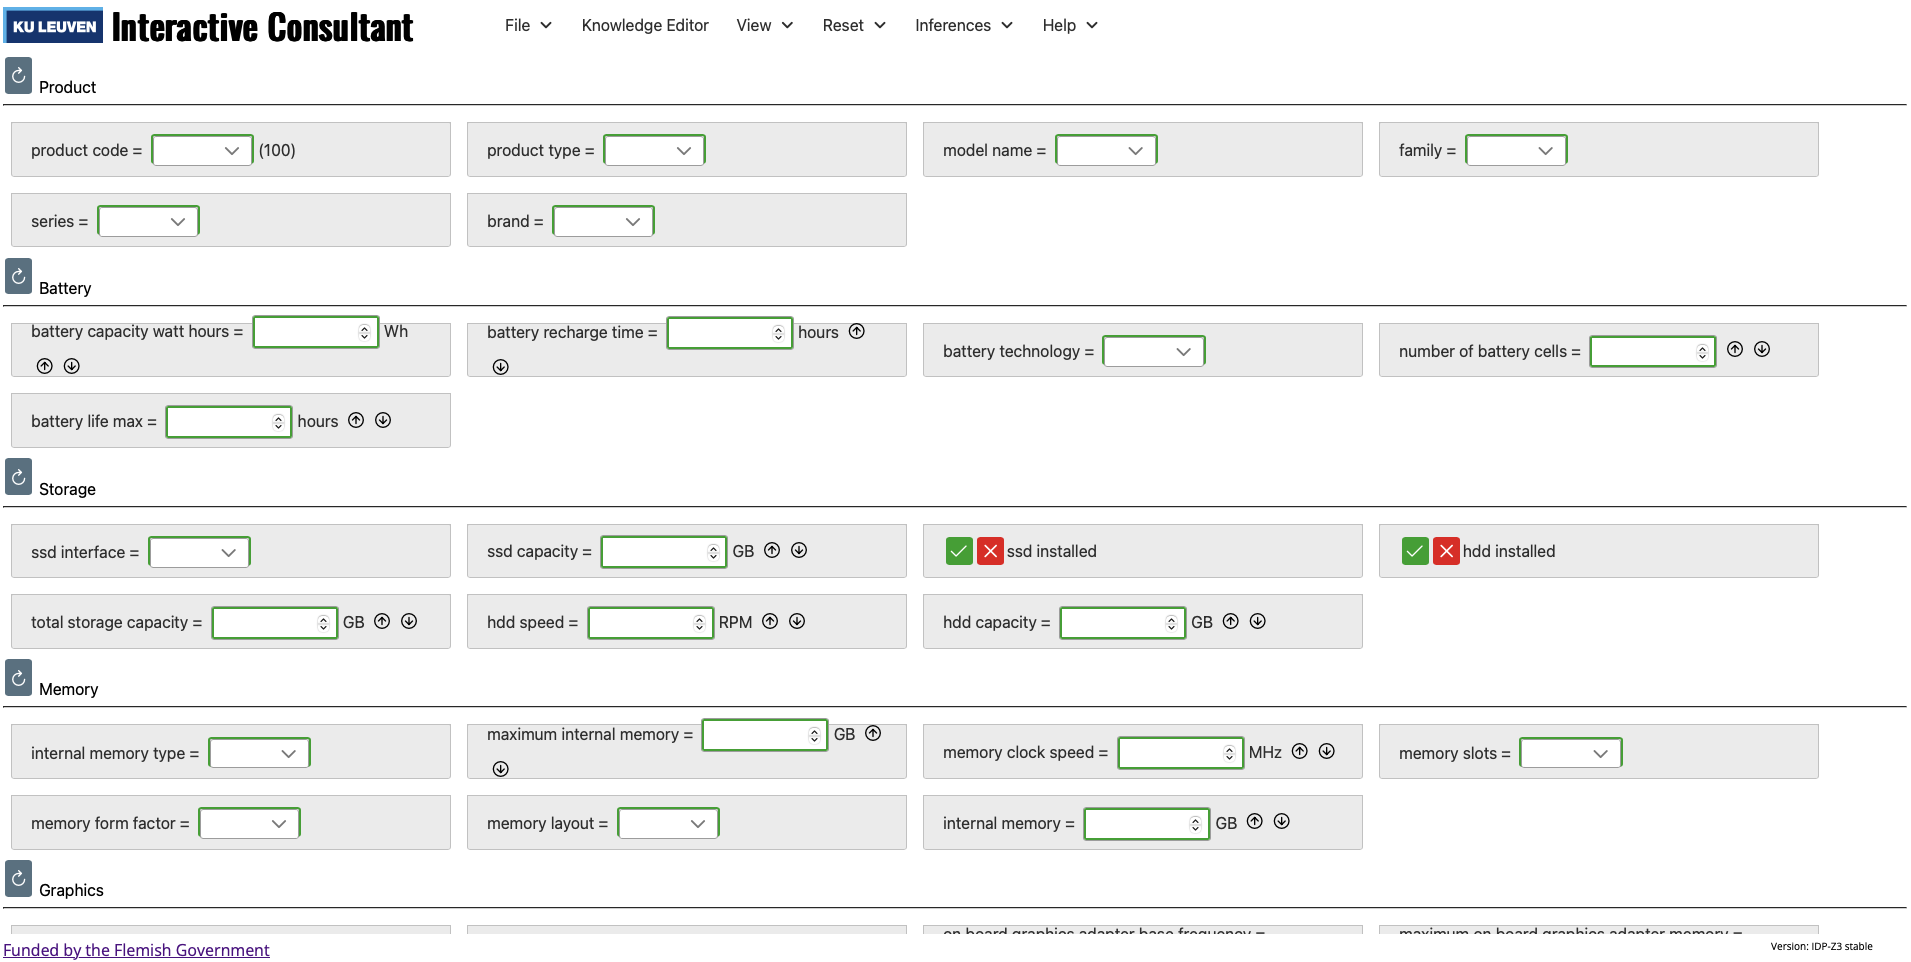
\includegraphics[width=1\textwidth]{gui.png}
    \caption[Huidige gebruikersinterface.]{\label{fig:gui}De online shop voor laptops in de Interactive Consultant~\autocite{KULeuven}.}
\end{figure}

\subsection{Frontend - GUI}
Voor dit onderzoek wordt er gekeken naar de grafische gebruikersinterface van een online shop voor laptops. De grafische user interface is uitgewerkt in Angular, een TypeScript-based open-source front-end framework dat ontwikkeld is door Google. Er wordt gebruik gemaakt van de PrimeNG UI-componentenbibliotheek. Deze library biedt een verzameling van herbruikbare componenten.

\subsubsection{Opbouw GUI}
\paragraph{Header}
De header bevat het KU Leuven-logo, een titel en een menubalk, en blijft behouden in de nieuwe UI (zie Figuur \ref{fig:header}).

\begin{figure}
  \centering
  
\includegraphics[width=1\textwidth]{header.png}
  \caption[Header huidige en nieuwe UI.]{\label{fig:header}De header van de Interactive Consultant met alle componenten~\autocite{KULeuven}.}
\end{figure}

\paragraph{ScrollPanel}
De content van de pagina zit vervat in een ScrollPanel. Deze scrollcontainer is opgedeeld in rijachtige structuur voor elke categorie van properties (zie Figuur \ref{fig:scrollpanel}).

\begin{figure}
    \centering
    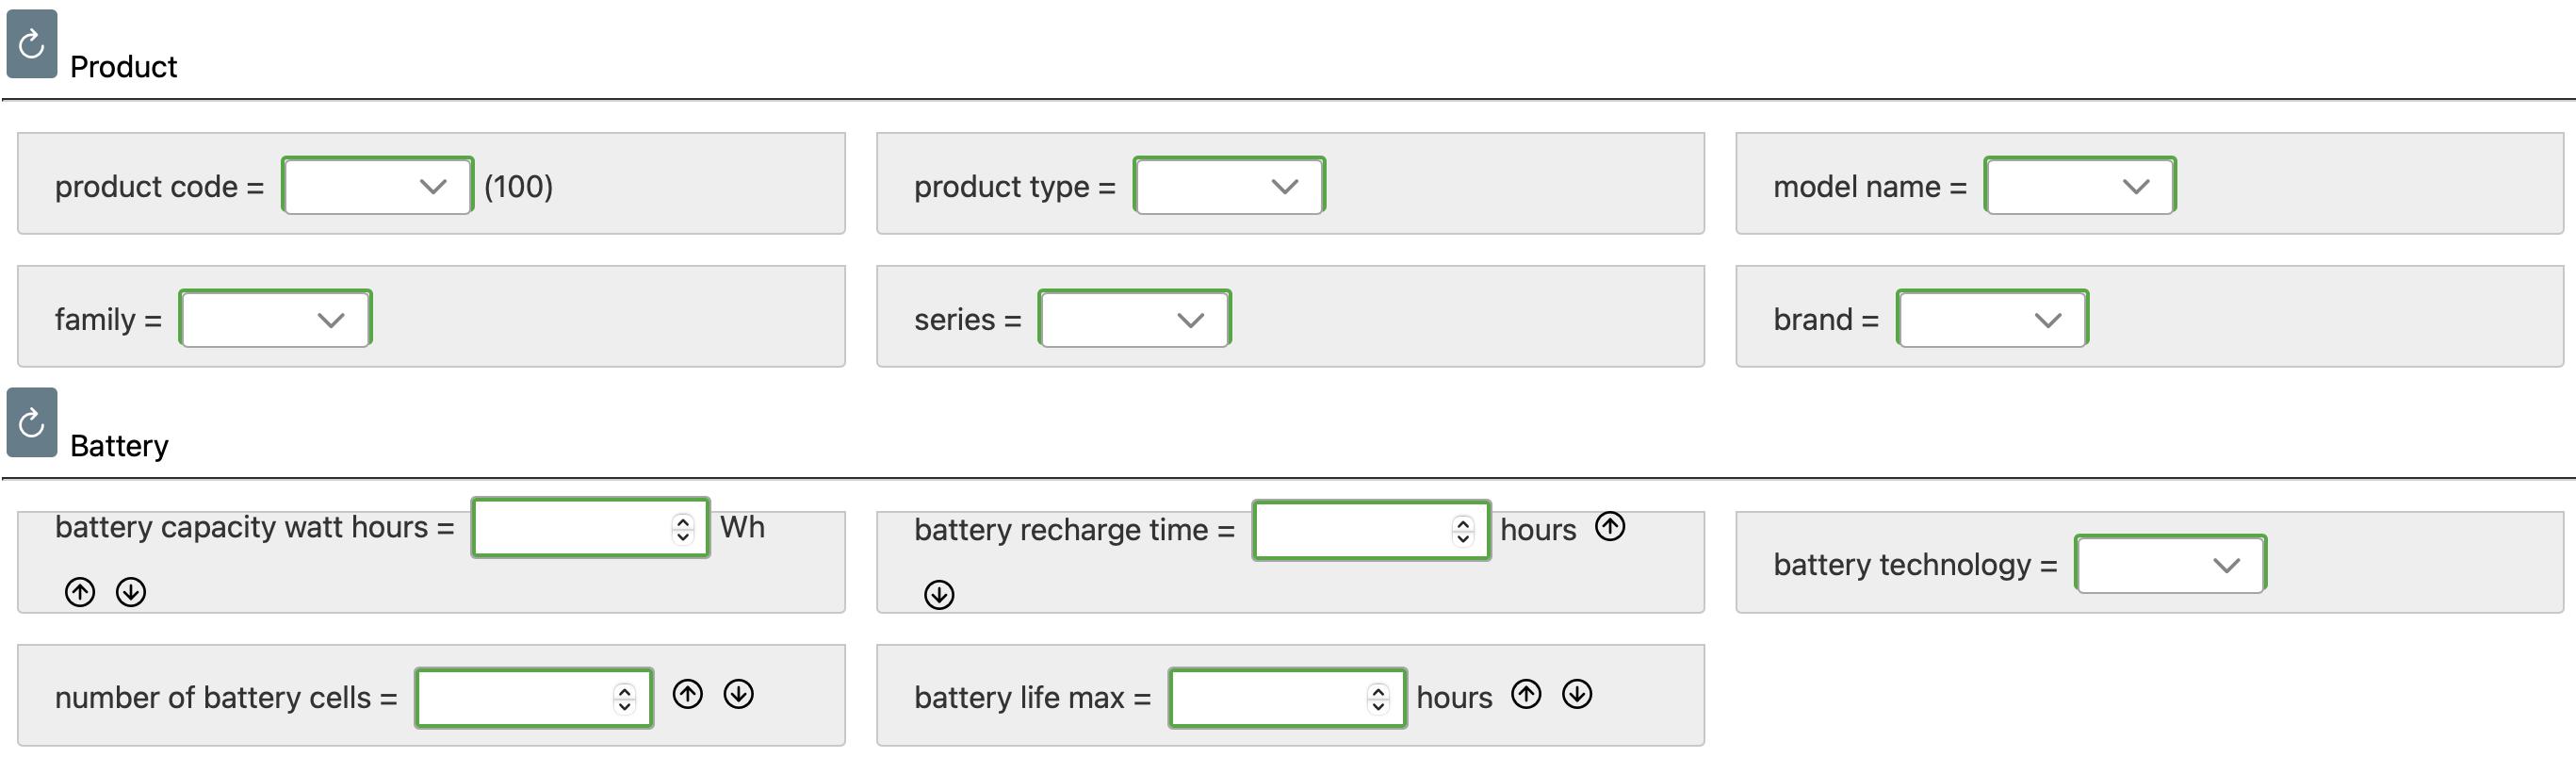
\includegraphics[width=1\textwidth]{scrollpanel.png}
    \caption[ScrollPanel van huidige UI]{\label{fig:scrollpanel}De content van de ScrollPanel opgedeeld in rijen op basis van de categorie van een property. In bovenstaande afbeelding zijn properties uit categorieën \textit{Product} en \textit{Battery} te zien~\autocite{KULeuven}.}
\end{figure}

\paragraph{Dropdown, binaire keuzeselector en invoerveld}
De properties worden weergegeven als dropdowns, binaire keuzeselectoren of invoervelden, afhankelijk van het type keuze dat de gebruiker moet maken. Dropdowns worden gebruikt wanneer er meerdere opties beschikbaar zijn, terwijl binaire keuzeselectoren geschikt zijn voor beslissingen met slechts twee mogelijke waarden, zoals ja/nee of aan/uit. De invoervelden zijn van het type number, waarbij zowel gehele als decimale waarden kunnen worden ingevoerd. In figuur \ref{fig:componenten} worden de drie UI-componenten afgebeeld.

\begin{figure}
    \centering
    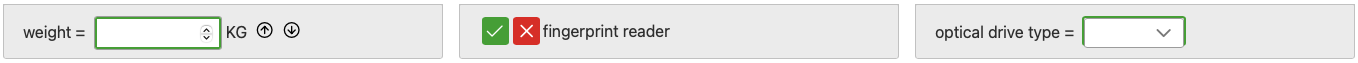
\includegraphics[width=1\textwidth]{componenten.png}
    \caption[Dropdown, binaire keuzeselector en invoerveld]{\label{fig:componenten}Voor property \textit{weight} wordt  een numeriek invoerveld gebruikt, terwijl voor property \textit{fingerprint reader} een binaire keuzeselector wordt toegepast. De property \textit{optical drive type} wordt voorgesteld met een dropdown~\autocite{KULeuven}.}
\end{figure}

\subsection{Backend - Technisch}
\subsubsection{IDP-Z3}
IDP-Z3 is een redeneersysteem dat het Knowledge Base-paradigma implementeert met behulp van de FO[·]-taal. FO[·], ook bekend als FO-dot, is Eerste-Orde Logica waarmee kennis over een specifiek probleemgebied wordt vastgelegd. Deze kennis wordt vervolgens gebruikt om die problemen op te lossen door middel van redeneringen~\autocite{Carbonnelle2024}. Meer informatie over IDP-Z3 en de werking ervan is terug te vinden in de documentatie van~\textcite{Carbonnelle2024}.

\subsubsection{Properties}
De properties worden ingeladen met een JSON-bericht. Wanneer een gebruiker een wijziging aanbrengt in een veld, wordt het systeem opnieuw berekend en wo\-rdt er een nieuw JSON-bestand naar de IC gestuurd. De IC communiceert continu met IDP-Z3 om tot een oplossing te komen.

\subsubsection{Datamodel}
Er is geen persistente opslag van de ingevoerde gegevens, wat betekent dat deze niet bewaard blijven tussen sessies of voor toekomstige gebruik. Omdat de backend alles opnieuw berekent, is er geen sprake van een klassiek datamodel waarin gegevens kunnen worden opgeslagen en later opgehaald. Dit maakt het systeem flexibel en zorgt ervoor dat het altijd met de meest actuele gegevens werkt, maar betekent ook dat er geen historisch overzicht of hergebruik van gegevens mogelijk is. Dit laatste aspect is van cruciaal belang voor de nieuwe gebruikersinterface.

\section{Requirements-analysefase}
Bij het ontwikkelen van een nieuwe gebruikersinterface is het belangrijk te weten waaraan deze moet voldoen. Hiervoor worden zowel de functionele als niet-functionele vereisten geformuleerd. Daarnaast worden ze geordend volgens prioriteit, gebruik makend van de MoSCoW-methode. Deze fase kan beschouwd worden als de start van de vergelijken\-de studie van beschikbare technologieën en bibliotheken.

\subsection{Functionele vereisten}
Deze vereisten beschrijven de functionaliteit die het systeem moet bieden, oftewel de functies die de interface moet ondersteunen om de gebruiker te helpen.

\subsubsection{Must have}
\paragraph{Selecteren van properties}
Een gebruiker moet op properties kunnen klikken om een waarde in te vullen voor de gekozen property of om de verklaring te krijgen waarom een waarde al is gekozen of ingevuld.

\paragraph{Geselecteerde properties bijhouden}
De geselecteerde properties moeten worden bijgehouden en apart weergegeven.

\paragraph{Deselecteren van properties}
Een gebruiker moet eerder gemaakte keuzes, zowel door zichzelf als door het systeem, ongedaan kunnen maken door een property te deselecteren. De waarde van de property moet worden gereset, zodat de betreffende property niet meer wordt bijgehouden of greyed out is.

\paragraph{Resetten van properties}
Een gebruiker moet de waarden van alle properties kunnen resetten.

\paragraph{Real-time feedback}
De interface moet de gevolgen van de selecties van een gebruiker weergeven en moet kunnen verduidelijken waarom bepaalde keuzes automatisch worden toegepast. Een gebruiker moet dus directe feedback krijgen voor elke keuze die hij maakt.

\paragraph{Opslaan klikgedrag en visuele indicaties}
Het systeem moet bijhouden welke properties door gebruikers worden aangeklikt, samen met de bijhorende relevantie. Wanneer een gebruiker een keuze ongedaan maakt door een property te deselecteren, moet het systeem de relevantie van die property opnieuw aanpassen. Op basis van deze relevantie bepaalt het systeem een gewicht of grootte voor elke property. Properties die frequent worden aangeklikt, worden groter en opvallender weergegeven. Het systeem werkt de weergave van de properties dagelijks bij.

\paragraph{Begeleiding}
De opgeslagen informatie van de properties wordt gebruikt om gerichte aanbevelingen te doen aan gebruikers. De interface moet vrijblijvende hulp en begeleiding bieden zonder de vrijheid van de gebruiker te beperken. Dit is belangrijk, aangezien de huidige interface geen ondersteuning biedt.

\paragraph{Visuele hiërarchie en uitlijning}
De interface moet een duidelijke visuele hiërarchie en uitlijning hebben, met een logische en compacte structuur voor de presentatie van gegevens, zodat de gebruiker niet wordt overrompeld door te veel informatie. Dit is essentieel, omdat dit momenteel het probleem is van de bestaande gebruikersinterface.

\paragraph{Eenvoudige navigatie}
De interface moet een eenvoudig navigatiepad bieden, zodat een gebruiker snel de gewenste informatie kan vinden en te allen tijde weet waar hij zich binnen de interface bevindt.

\paragraph{Backend integratie met IDP-Z3}
Het systeem moet in staat zijn om te communiceren met IDP-Z3, wat momenteel gebeurt op basis van JSON-berichten. Deze werkwijze moet behouden blijven.

\subsubsection{Should have}
\paragraph{Hoveren over properties}
Een gebruiker moet over properties kunnen hoveren om meer uitleg te krijgen over wat de betreffende property inhoudt.

\subsection{Niet-functionele vereisten}
Deze vereisten beschrijven hoe het systeem de functionele vereisten moet uitvoeren. 

\subsubsection{Must have}
\paragraph{Gebruiksvriendelijkheid}
De interface moet gebruiksvriendelijk zijn, zonder onnodige complexiteit en intuïtief aanvoelen, zodat een gebruiker er vlot mee kan werken.

\paragraph{Esthetiek en visueel design}
De interface moet een aantrekkelijke visuele laag bieden die de gebruiker niet alleen ondersteunt, maar ook een aangename ervaring biedt. Het design moet consistent, responsive en modern zijn.

\paragraph{Gebruik van kleuren}
De interface gebruikt kleuren om aan te geven welke properties relevant zijn en welke niet.

\subsubsection{Should have}
\paragraph{Prestaties}
De interface moet snel reageren op gebruikersinvoer en zonder merkbare vertraging worden bijgewerkt.

\section {Long list fase}
Dit onderzoek bouwt voort op een reeds bestaand en actief project. De huidige webclient is ontwikkeld met Angular, een JavaScript-gebaseerd framework. In deze fase wordt er onderzocht welke softwarebibliotheken, binnen JavaScript of Angular zelf, geschikt zijn voor dit onderzoek. De focus ligt op libraries die gunstig zijn voor data- of tekstvisualisatie, aangezien het met de nieuwe webclient mogelijk moet zijn om woorden op een elegante en compacte manier weer te geven in verschillenden kleuren en groottes.\smallskip\par
Binnen een library zijn vaak meerdere visualisatiemethoden beschikbaar. De insteek van deze bachelorproef was initieel om te onderzoeken of het mogelijk is een woordwolk te implementeren als nieuwe gebruikersinterface. Deze vergelijkende studie gaat echter breder dan alleen libraries voor woordwolken. Uit onderzoeken van~\textcite{Wang2015} worden er volgende categorieën van datavisualisatietechnieken aangehaald: grafieken, netwerken en hiërarchieën.\par Vooraleer een keuze wordt gemaakt, wordt de literatuur doorzocht naar alternatieven binnen deze drie categorieën.

\subsection{Gevonden alternatieven}
\subsubsection{D3.js}
D3.js is een open-sourcebibliotheek die zich richt op animaties, interacties en dynamische visualisaties. De nadruk ligt op de efficiënte manipulatie van HTML-eleme\-ten. Standaard genereert D3.js geen voorgedefinieerde visualisaties; de functionaliteit moet daarom worden uitgebreid met plug-ins of externe bibliotheken. De bibliotheek biedt een breed scala aan lay-outs voor verschillende soorten data~\autocite{Wang2015}.
\subsubsection{Sigma.js}
Sigma.js is een open-sourcebibliotheek die in staat is dynamische interactieve grafen te tekenen. Deze library is makkelijk inzetbaar en kan vlot worden geïntegreerd in bestaande webtoepassingen. De standaardinstellingen van de bibliotheek bevatten diverse ingebouwde functies, waaronder ondersteuning voor muis- en aanraakbediening~\autocite{Wang2015}.
\subsubsection{Cytoscape.js}
Cytoscape.js is een open-sourcebibliotheek ontworpen voor het visualiseren van grafen. Het ondersteunt verschillende gebruikersinteracties zoals selecteren en pannen~\autocite{Wang2015}.
\subsubsection{Highcharts}
Highcharts is een open-sourcebibliotheek die ondersteuning biedt voor interactieve grafieken op basis van CSV- en JSON-data~\autocite{Vucetic2023}. De library beschikt over een eigen chatbot, wat het vergemakkelijkt om snel informatie op te zoeken en problemen op te lossen~\autocite{Highcharts2025}.
\subsubsection{amCharts}
amCharts is een hulpmiddel voor het visualiseren van complexe data via interactieve grafieken en kaarten. Standaard wordt data geleverd via een array die in de JavaScript-code is opgenomen, maar voor geavanceerdere toepassingen kunnen ook andere databronnen worden gebruikt~\autocite{Chandra2022}.
\subsubsection{Vega}
Vega functioneert als een raamwerk voor datavisualisatie. Het visuele uiterlijk en het interactieve gedrag wordt gedefinieerd aan de hand van JSON~\autocite{Chandra2022}. 
\subsubsection{ZingChart}
ZingChart biedt ontwikkelaars een oplossing voor het creëren van responsieve visualisaties~\autocite{Chandra2022}.
\medskip\par
Naast het raadplegen van wetenschappelijke en professionele bronnen, wordt er ook gezocht naar open-source GitHub-bibliotheken voor woordwolkvisualisaties. Hierbij is volgende alternatief gevonden:
\begin{itemize}
    \item \textbf{Wordcloud2.js}: een standalone library van Timothy Guan-tin Chien~\autocite{Chien2011}.
\end{itemize}

\subsection{Toetsen requirements}
In dit deel van de fase worden de officiële websites en documentatie van elk alternatief zijn grondig bestudeerd. Vooraleer de vereisten geëvalueerd en getoetst kunnen worden, is het essentieel om eerst te bepalen welke visualisaties het meest geschikt en relevant zijn voor dit onderzoek. De nieuwe interface moet gestructureerd, overzichtelijk, compact, intuïtief én visueel aantrekkelijk zijn. Bepaalde visualisatietypes zoals lijn-, staaf- en kolomgrafieken, worden uitgesloten. Na een grondige analyse van de mogelijke visualisaties binnen de bibliotheken uit de long list, blijken de volgende structuren geschikt voor dit onderzoek: een woordwolk, een (packed) bubble chart en een graaf.\medskip\par
Om de requirements op een correcte manier te kunnen toetsen, moet eerst technisch worden nagedacht over hoe elke vereiste geïmplementeerd kan worden. Da\-arbij wordt binnen de softwarebibliotheken gezocht naar functionaliteiten die standaard door de library worden aangeboden. Dit zijn de gewenste eigenschappen:
\begin{itemize}
    \item \textbf{Klik functie}: de gebruiker moet op een woord kunnen klikken om er een waarde aan toe te kennen.
    \item \textbf{State management}: de gebruiker moet een overzicht kunnen zien van de woorden waaraan hij al een waarde heeft toegekend.
    \item \textbf{(Re)render functie}: de visualisatie moet zich kunnen aanpassen of opnieuw laden op basis van de interacties van de gebruiker.
    \item \textbf{Gebruik van verschillende kleuren binnen de visualisatie}: kleuren bieden visuele begeleiding, geven betekenis en zorgen voor een aangename uitstraling.
    \item \textbf{Gebruik van verschillende tekstgroottes binnen de visualisatie}: variatie in tekstgrootte ondersteunt visuele hiërarchie, structuur en leesbaarheid.
    \item \textbf{Hover functie}: de gebruiker moet met de muis over een woord kunnen bewegen om extra informatie over dat woord te verkrijgen.
\end{itemize}

De vereisten in de tabellen zijn gerangschikt volgens de volgorde zoals gedefinieerd in de requirementsanalysefase. Deze structuur wordt in de tabel weergegeven met een horizontale oriëntatie, waarbij de vereisten van links naar rechts worden gepresenteerd.

\paragraph{D3.js - Woordwolk}
Uit de documentatie van~\textcite{D3Contributors2025} en~\textcite{Mike2025} blijkt dat D3.js, en dus ook de woordwolkcomponent, ingebouwde klik- en hoverfunctionaliteiten biedt. Dit houdt in dat zowel het selecteren en deselecteren van eigenschappen als het tonen van extra informatie bij een woord wordt ondersteund. Het opslaan van klikgedrag is mogelijk, waardoor een relevantieverschil tussen eigenschappen kan worden opgebouwd. Ook het instellen van verschillende kleuren en tekstgroottes per woord is ondersteund. Bovendien kan D3.js goed overweg met JSON-data. Deze visualisatie maakt het dus mogelijk om visuele indicaties, begeleiding en hiërarchie te implementeren. Hoewel het bijhouden van geselecteerde properties niet standaard wordt voorzien binnen D3.js, kan deze functionaliteit wel eenvoudig worden toegevoegd via state management binnen het gebruikte JavaScript-framework.

\begin{table}[htbp]
    \centering
    \begin{minipage}{0.48\textwidth}
        \centering
        \begin{tabular}{|ccccccccc|c|}
            \hline
            \multicolumn{9}{|c|}{M} & \multicolumn{1}{c|}{S} \\
            \midrule
            $\bullet$ & --- & $\bullet$ & $\bullet$ & $\bullet$ & $\bullet$ & $\bullet$ & $\bullet$ & $\bullet$ & $\bullet$ \\
            \bottomrule
        \end{tabular}
        \caption{D3.js Woordwolk - Functionele requirements}
    \end{minipage}
    \hfill
    \begin{minipage}{0.48\textwidth}
        \centering
        \begin{tabular}{|ccc|c|}
            \hline
            \multicolumn{3}{|c|}{M} & \multicolumn{1}{c|}{S} \\
            \midrule
            $\bullet$ & $\bullet$ & $\bullet$ & ? \\
            \bottomrule
        \end{tabular}
        \caption{D3.js Woordwolk - Niet-functionele requirements}
    \end{minipage}
    \caption*{($\bullet$ = req aanwezig; --- = req niet aanwezig; ? = geen info beschikbaar)}
\end{table}

\paragraph{D3.js - Bubble Chart}
Uit de documentatie van~\textcite{D3Contributors2025} en~\textcite{Mike2025a} blijkt dat de bubble chart-visualisatie sterk gelijkt op de woordwolk. Er is echter een duidelijk visueel verschil tussen beide libraries. Woordwolken gebruiken tekst als primair visueel element, met variaties in grootte, kleur en oriëntatie. Bubble charts daarentegen maken gebruik van cirkels als primair visueel element, waarbij tekst meestal een secundaire rol speelt. Het bijhouden van geselecteerde eigenschappen is ook in dit geval niet standaard voorzien binnen D3.js, maar deze functionaliteit kan worden toegevoegd via state management binnen het gebruikte JavaScript-framework.

\begin{table}[htbp]
    \centering
    \begin{minipage}{0.48\textwidth}
        \centering
        \begin{tabular}{|ccccccccc|c|}
            \hline
            \multicolumn{9}{|c|}{M} & \multicolumn{1}{c|}{S} \\
            \midrule
            $\bullet$ & --- & $\bullet$ & $\bullet$ & $\bullet$ & $\bullet$ & $\bullet$ & $\bullet$ & $\bullet$ & $\bullet$ \\
            \bottomrule
        \end{tabular}
        \caption{D3.js Bubble Chart - Functionele requirements}
    \end{minipage}
    \hfill
    \begin{minipage}{0.48\textwidth}
        \centering
        \begin{tabular}{|ccc|c|}
            \hline
            \multicolumn{3}{|c|}{M} & \multicolumn{1}{c|}{S} \\
            \midrule
            $\bullet$ & $\bullet$ & $\bullet$ & ? \\
            \bottomrule
        \end{tabular}
        \caption{D3.js Bubble Chart - Niet-functionele requirements}
    \end{minipage}
    \caption*{($\bullet$ = req aanwezig; --- = req niet aanwezig; ? = geen info beschikbaar)}
\end{table}

Wanneer er met grote datasets wordt gewerkt, kan een bubble chart onoverzichtelijk worden omdat deze niet meer binnen de schermgrootte past of niet volledig in één scherm weergegeven kan worden. Bubbels die zeer relevante woorden bevatten, kunnen namelijk snel te groot worden, terwijl tekst alleen minder ruimte inneemt.

\paragraph{Sigma.js - Graaf}
Uit de documentatie van~\textcite{SigmaJS2025} blijkt dat alle functionele requirements haalbaar zijn, met uitzondering van het bijhouden van de geselecteerde properties. Er zijn voldoende ondersteunde events beschikbaar, zoals klik-, enter- en leaveNode-events. Sigma.js zorgt ervoor dat de volledige graaf zichtbaar is en benut de beschikbare ruimte efficiënt. Een interessante functionaliteit van Sigma.js in het kader van dit onderzoek is de mogelijkheid om vlak vóór het renderen de eigenschappen van nodes dynamisch aan te passen.

\begin{table}[htbp]
    \centering
    \begin{minipage}{0.48\textwidth}
        \centering
        \begin{tabular}{|ccccccccc|c|}
            \hline
            \multicolumn{9}{|c|}{M} & \multicolumn{1}{c|}{S} \\
            \midrule
            $\bullet$ & --- & $\bullet$ & $\bullet$ & $\bullet$ & $\bullet$ & $\bullet$ & $\bullet$ & $\bullet$ & $\bullet$ \\
            \bottomrule
        \end{tabular}
        \caption{Sigma.js - Functionele requirements}
    \end{minipage}
    \hfill
    \begin{minipage}{0.48\textwidth}
        \centering
        \begin{tabular}{|ccc|c|}
            \hline
            \multicolumn{3}{|c|}{M} & \multicolumn{1}{c|}{S} \\
            \midrule
            ? & $\bullet$ & $\bullet$ & ? \\
            \bottomrule
        \end{tabular}
        \caption{Sigma.js - Niet-functionele requirements}
    \end{minipage}
    \caption*{($\bullet$ = req aanwezig; --- = req niet aanwezig; ? = geen info beschikbaar)}
\end{table}

\paragraph{Cytoscape.js - Graaf}
Het artikel van~\textcite{Franz2015} en de documentatie van Cytoscape.js~\textcite{Franz2025} geven aan dat de functionaliteiten van de library aan de meeste requirements voldoen. Opnieuw is er geen ingebouwde mogelijkheid om de geselecteerde properties bij te houden. Cytoscape.js maakt real-time feedback mogelijk dankzij de functionaliteit om elementen dynamisch toe te voegen, te verwijderen of te wijzigen. Daarnaast kunnen stylesheets tijdens runtime worden vervangen om de visuele stijl aan te passen. Deze library biedt ondersteuning voor JSON-import en -export, wat de integratie met backend-systemen zoals het IDP-Z3-syst\-eem mogelijk maakt. Ook gebruikersinteracties zoals klikken en hoveren kunnen worden afgehandeld. Een nuttige functionaliteit in het kader van dit onderzoek is dat de visualisatie automatisch wordt gerenderd wanneer nodig.

\begin{table}[htbp]
    \centering
    \begin{minipage}{0.48\textwidth}
        \centering
        \begin{tabular}{|ccccccccc|c|}
            \hline
            \multicolumn{9}{|c|}{M} & \multicolumn{1}{c|}{S} \\
            \midrule
            $\bullet$ & --- & $\bullet$ & $\bullet$ & $\bullet$ & $\bullet$ & $\bullet$ & $\bullet$ & $\bullet$ & $\bullet$ \\
            \bottomrule
        \end{tabular}
        \caption{Cytoscape.js - Functionele requirements}
    \end{minipage}
    \hfill
    \begin{minipage}{0.48\textwidth}
        \centering
        \begin{tabular}{|ccc|c|}
            \hline
            \multicolumn{3}{|c|}{M} & \multicolumn{1}{c|}{S} \\
            \midrule
            ? & $\bullet$ & $\bullet$ & $\bullet$ \\
            \bottomrule
        \end{tabular}
        \caption{Cytoscape.js - Niet-functionele requirements}
    \end{minipage}
    \caption*{($\bullet$ = req aanwezig; --- = req niet aanwezig; ? = geen info beschikbaar)}
\end{table}

\paragraph{Highcharts - Woordwolk}
Volgens de website en documentatie van~\textcite{Highcharts2009,Highcharts2009a} biedt de module zowel ingebouwde klik- als hoverfunctionaliteit, waardoor gebruikersinteracties kunnen worden afgehandeld. Daarnaast is het mogelijk om tekstgroottes en kleuren per woord aan te passen, wat belangrijk is voor het visualiseren van prioriteit en categorieën. Highcharts heeft een functie \textit{redraw} waardoor de woordwolk opnieuw wordt gerenderd. Highcharts kan overweg met JSON-data, maar heeft geen ingebouwde mogelijkheid voor het bijhouden van geselecteerde properties. Dit kan worden opgelost binnen de Angular-omgeving.

\begin{table}[htbp]
    \centering
    \begin{minipage}{0.48\textwidth}
        \centering
        \begin{tabular}{|ccccccccc|c|}
            \hline
            \multicolumn{9}{|c|}{M} & \multicolumn{1}{c|}{S} \\
            \midrule
            $\bullet$ & --- & $\bullet$ & $\bullet$ & $\bullet$ & $\bullet$ & $\bullet$ & $\bullet$ & $\bullet$ & $\bullet$ \\
            \bottomrule
        \end{tabular}
        \caption{Highcharts Woordwolk - Functionele requirements}
    \end{minipage}
    \hfill
    \begin{minipage}{0.48\textwidth}
        \centering
        \begin{tabular}{|ccc|c|}
            \hline
            \multicolumn{3}{|c|}{M} & \multicolumn{1}{c|}{S} \\
            \midrule
            ? & $\bullet$ & $\bullet$ & ? \\
            \bottomrule
        \end{tabular}
        \caption{Highcharts Woordwolk - Niet-functionele requirements}
    \end{minipage}
    \caption*{($\bullet$ = req aanwezig; --- = req niet aanwezig; ? = geen info beschikbaar)}
\end{table}

\paragraph{Highcharts - Packed Bubble Chart}
Net als bij de woordwolk ondersteunt de packed bubble chart klik- en hoverfuncties, en kunnen zowel kleuren als groottes aangepast worden op basis van de data. Beide visualisaties binnen Highcharts vertonen sterke gelijkenissen qua functionaliteit, maar verschillen in visuele presentatie. In tegenstelling tot de woordwolk maakt de packed bubble chart gebruik van cirkels, waarbij de grootte van elke cirkel wordt bepaald door de relevantie van de property~\autocite{Highcharts2009,Highcharts2009a}.

\begin{table}[htbp]
    \centering
    \begin{minipage}{0.48\textwidth}
        \centering
        \begin{tabular}{|ccccccccc|c|}
            \hline
            \multicolumn{9}{|c|}{M} & \multicolumn{1}{c|}{S} \\
            \midrule
            $\bullet$ & --- & $\bullet$ & $\bullet$ & $\bullet$ & $\bullet$ & $\bullet$ & $\bullet$ & $\bullet$ & $\bullet$ \\
            \bottomrule
        \end{tabular}
        \caption{Highcharts Packed Bubble Chart - Functionele requirements}
    \end{minipage}
    \hfill
    \begin{minipage}{0.48\textwidth}
        \centering
        \begin{tabular}{|ccc|c|}
            \hline
            \multicolumn{3}{|c|}{M} & \multicolumn{1}{c|}{S} \\
            \midrule
            ? & $\bullet$ & $\bullet$ & ? \\
            \bottomrule
        \end{tabular}
        \caption{Highcharts Packed Bubble Chart - Niet-functionele requirements}
    \end{minipage}
    \caption*{($\bullet$ = req aanwezig; --- = req niet aanwezig; ? = geen info beschikbaar)}
\end{table}
\paragraph{amCharts - Woordwolk}
Uit de documentatie van~\textcite{amCharts2025} blijkt dat de woordwolkcomponent zeer flexibel is en tal van interactieve mogelijkheden biedt. Zo ondersteunt de bibliotheek zowel klik- als hoverfunctionaliteiten en laat ze toe om eigenschappen zoals grootte, kleur en positie van woorden dynamisch aan te passen. Daarnaast beschikt amCharts over geavanceerde animatieopties, wat zorgt voor een aantrekkelijke en gebruiksvriendelijke interface. De duidelijke ondersteuning voor JSON-data maakt het bovendien eenvoudig om te koppelen met de backend. De library biedt opnieuw geen ingebouwde state management voor het bijhouden van geselecteerde properties. Volgens~\textcite{Ravishankkar2017} heeft amCharts ook geen prestatieproblemen.

\begin{table}[htbp]
    \centering
    \begin{minipage}{0.48\textwidth}
        \centering
        \begin{tabular}{|ccccccccc|c|}
            \hline
            \multicolumn{9}{|c|}{M} & \multicolumn{1}{c|}{S} \\
            \midrule
            $\bullet$ & --- & $\bullet$ & $\bullet$ & $\bullet$ & $\bullet$ & $\bullet$ & $\bullet$ & $\bullet$ & $\bullet$ \\
            \bottomrule
        \end{tabular}
        \caption{amCharts Woordwolk - Functionele requirements}
    \end{minipage}
    \hfill
    \begin{minipage}{0.48\textwidth}
        \centering
        \begin{tabular}{|ccc|c|}
            \hline
            \multicolumn{3}{|c|}{M} & \multicolumn{1}{c|}{S} \\
            \midrule
            ? & $\bullet$ & $\bullet$ & $\bullet$ \\
            \bottomrule
        \end{tabular}
        \caption{amCharts Woordwolk - Niet-functionele requirements}
    \end{minipage}
    \caption*{($\bullet$ = req aanwezig; --- = req niet aanwezig; ? = geen info beschikbaar)}
\end{table}
\paragraph{Vega - Woordwolk}
De bibliotheek werkt met JSON-specificaties die de visualisatie en interacties definiëren. Uit de documentatie blijkt dat Vega ondersteuning biedt voor gebruikersinteracties zoals klikken en hoveren, en dat de visualisatie kan worden aangepast op basis van dynamische data. Hoewel Vega zeer flexibel is, vereist het meer code en configuratie dan gespecialiseerde woordwolk-libraries. Het bijhouden van geselecteerde properties is niet ingebouwd en moet worden geïmplementeerd in de Angular-applicatie. Volgens het onderzoek van~\textcite{Satyanarayan2017} is de interactieve performance van Vega minstens twee keer zo snel als die van een gelijkwaardig D3-programma.
\begin{table}[htbp]
    \centering
    \begin{minipage}{0.48\textwidth}
        \centering
        \begin{tabular}{|ccccccccc|c|}
            \hline
            \multicolumn{9}{|c|}{M} & \multicolumn{1}{c|}{S} \\
            \midrule
            $\bullet$ & --- & $\bullet$ & $\bullet$ & $\bullet$ & $\bullet$ & $\bullet$ & $\bullet$ & $\bullet$ & $\bullet$ \\
            \bottomrule
        \end{tabular}
        \caption{Vega Woordwolk - Functionele requirements}
    \end{minipage}
    \hfill
    \begin{minipage}{0.48\textwidth}
        \centering
        \begin{tabular}{|ccc|c|}
            \hline
            \multicolumn{3}{|c|}{M} & \multicolumn{1}{c|}{S} \\
            \midrule
            ? & $\bullet$ & $\bullet$ & $\bullet$ \\
            \bottomrule
        \end{tabular}
        \caption{Vega Woordwolk - Niet-functionele requirements}
    \end{minipage}
    \caption*{($\bullet$ = req aanwezig; --- = req niet aanwezig; ? = geen info beschikbaar)}
\end{table}
\paragraph{Vega - Packed Bubble Chart}
De packed bubble chart visualisatie in Vega ondersteunt dezelfde functionaliteiten als de woordwolk. Ze verschillen enkel in visuele weergave.

\begin{table}[htbp]
    \centering
    \begin{minipage}{0.48\textwidth}
        \centering
        \begin{tabular}{|ccccccccc|c|}
            \hline
            \multicolumn{9}{|c|}{M} & \multicolumn{1}{c|}{S} \\
            \midrule
            $\bullet$ & --- & $\bullet$ & $\bullet$ & $\bullet$ & $\bullet$ & $\bullet$ & $\bullet$ & $\bullet$ & $\bullet$ \\
            \bottomrule
        \end{tabular}
        \caption{Vega Packed Bubble Chart - Functionele requirements}
    \end{minipage}
    \hfill
    \begin{minipage}{0.48\textwidth}
        \centering
        \begin{tabular}{|ccc|c|}
            \hline
            \multicolumn{3}{|c|}{M} & \multicolumn{1}{c|}{S} \\
            \midrule
            ? & $\bullet$ & $\bullet$ & $\bullet$ \\
            \bottomrule
        \end{tabular}
        \caption{Vega Packed Bubble Chart - Niet-functionele requirements}
    \end{minipage}
    \caption*{($\bullet$ = req aanwezig; --- = req niet aanwezig; ? = geen info beschikbaar)}
\end{table}
\paragraph{ZingChart - Woordwolk}
ZingChart bevat een renderfunctie waarmee verschillende renderopties kunnen worden meegegeven. Zowel klik- als hoverfunctionaliteit is mogelijk. Daarnaast geeft de documentatie aan dat de grootte, kleur en positie van woorden aangepast kunnen worden. Integratie met het backend-systeem is haalbaar, maar ingebouwd state management ontbreekt~\autocite{ZingChart2009}.
\begin{table}[htbp]
    \centering
    \begin{minipage}{0.48\textwidth}
        \centering
        \begin{tabular}{|ccccccccc|c|}
            \hline
            \multicolumn{9}{|c|}{M} & \multicolumn{1}{c|}{S} \\
            \midrule
            $\bullet$ & --- & $\bullet$ & $\bullet$ & $\bullet$ & $\bullet$ & $\bullet$ & $\bullet$ & $\bullet$ & $\bullet$ \\
            \bottomrule
        \end{tabular}
        \caption{ZingChart Woordwolk - Functionele requirements}
    \end{minipage}
    \hfill
    \begin{minipage}{0.48\textwidth}
        \centering
        \begin{tabular}{|ccc|c|}
            \hline
            \multicolumn{3}{|c|}{M} & \multicolumn{1}{c|}{S} \\
            \midrule
            ? & $\bullet$ & $\bullet$ & ? \\
            \bottomrule
        \end{tabular}
        \caption{ZingChart Woordwolk - Niet-functionele requirements}
    \end{minipage}
    \caption*{($\bullet$ = req aanwezig; --- = req niet aanwezig; ? = geen info beschikbaar)}
\end{table}

\paragraph{Wordcloud2.js - Woordwolk}
Uit de API-documentatie van~\textcite{Chien2011a} blijkt duidelijk welke functionaliteiten beschikbaar zijn binnen de woordwolk. De documentatie biedt een overzicht van de opties die kunnen worden meegegeven bij de configuratie. De woordwolk beschikt over ingebouwde klik- en hoverfuncties, en het is mogelijk om per woord een specifieke kleur en tekstgrootte toe te kennen. De library is eenvoudig te integreren en vereist minimale configuratie voor basisfunctionaliteit. WordCloud2.js werkt met arrays van woorden en gewichten, wat compatibel is met de JSON-data die het backend-systeem aanlevert. Net als bij de andere libraries is er echter geen ondersteuning voor het bijhouden van geselecteerde properties.
\begin{table}[htbp]
    \centering
    \begin{minipage}{0.48\textwidth}
        \centering
        \begin{tabular}{|ccccccccc|c|}
            \hline
            \multicolumn{9}{|c|}{M} & \multicolumn{1}{c|}{S} \\
            \midrule
            $\bullet$ & --- & $\bullet$ & $\bullet$ & $\bullet$ & $\bullet$ & $\bullet$ & $\bullet$ & $\bullet$ & $\bullet$ \\
            \bottomrule
        \end{tabular}
        \caption{Wordcloud2.js Woordwolk - Functionele requirements}
    \end{minipage}
    \hfill
    \begin{minipage}{0.48\textwidth}
        \centering
        \begin{tabular}{|ccc|c|}
            \hline
            \multicolumn{3}{|c|}{M} & \multicolumn{1}{c|}{S} \\
            \midrule
            $\bullet$ & $\bullet$ & $\bullet$ & $\bullet$ \\
            \bottomrule
        \end{tabular}
        \caption{Wordcloud2.js Woordwolk - Niet-functionele requirements}
    \end{minipage}
    \caption*{($\bullet$ = req aanwezig; --- = req niet aanwezig; ? = geen info beschikbaar)}
\end{table}
\medskip\par Voor dit onderzoek mag geen enkele library prestatieproblemen vertonen, aangezien het prototype geen grote dataset hoeft te verwerken.

\section {Short list fase}
Uit de longlistfase kan geconcludeerd worden dat de besproken alternatieven sterk op elkaar lijken en grotendeels vergelijkbare functionaliteiten bieden. Het meest opvallende patroon is dat geen van de bibliotheken native ondersteuning biedt voor het bijhouden van geselecteerde properties. In dit onderzoek wordt er verdergegaan met de lichtgewicht, standalone library Wordcloud2.js. Een van de doelstellingen van deze studie is te onderzoeken of het mogelijk is om een woordwolk te integreren in de huidige webinterface. Aangezien deze library eenvoudig te integreren is en beschikt over duidelijke documentatie, vormt ze een geschikt alternatief.

\section{Architectuur van de nieuwe gebruikersinterface}
Een softwarebibliotheek is niet voldoende om een nieuwe gebruikersinterface te bouwen. De architectuur van de nieuwe gebruikersinterface moet ook besproken worden.

\subsection{Frontend}
Zoals hierboven reeds gezegd, is de frontend van de huidige webinterface ontwikkeld in Angular en blijft dit ongewijzigd. De gekozen softwarebibliotheek Wordcloud2.js wordt geïmplementeerd en gebruikt om een woordwolk te visualiseren.

\subsection{Backend IDP-Z3}
Het hele achterliggende redeneersysteem blijft ook behouden en ongewijzigd aangezien dit los staat van de nieuwe webinterface.

\subsection{Backend Node.js en Express}
Om het klikgedrag van de gebruiker op te slaan, is een REST API nodig. Wanneer de gebruiker een waarde toekent aan een property, wordt een HTTP-request verstuurd naar deze REST API om de interactie te registreren. Hiervoor wordt een backend opgezet met Node.js en Express in TypeScript, gebaseerd op een structuur die vergelijkbaar is met de tutorial van~\textcite{Mallawaarachchi2023}.

\subsection{PostgreSQL en PgAdmin}
De REST API heeft een databank nodig om de properties en interacties op te slaan. Er is gekozen voor de relationele databank PostgreSQL. Voor het beheren van deze databank wordt de grafische tool PgAdmin gebruikt.

\paragraph{Opmerking}
De keuze voor tools en frameworks zoals Express, Node.js en PostgreSQL is niet doorslaggevend voor dit onderzoek. Ze dienen enkel als hulpmiddelen om tot een oplossing te komen; hetzelfde resultaat kan ook met andere tools en frameworks worden bereikt.

\section{Proof-of-concept bouwen}
\subsection{Inlezen op huidige code}
Zoals vermeld in de verduidelijkingsfase bouwt dit onderzoek voort op een bestaand en actief project. De oorspronkelijke, volledige codebase is terug te vinden in de GitLab-repository van~\textcite{Carbonnelle2019}. Vooraleer er aanpassingen of uitbreidingen aan de code kunnen worden gedaan, is het belangrijk om eerst de relevante bestaande code te bestuderen en te begrijpen. Voor dit onderzoek wordt specifiek gekeken naar het deelproject idp\_web\_client, aangezien dit de code bevat voor de visualisatie en verwerking van de Interactive Consultant.

\subsection{Woordwolk visualisatie}
Eerst en vooral moet de library worden geïntegreerd in het project.
\begin{verbatim}npm install github:timdream/wordcloud2.js --save\end{verbatim}
Om de woordwolk effectief te kunnen gebruiken en aanroepen, moet deze worden geïmporteerd in het gewenste bestand.
\begin{verbatim}import WordCloud from 'wordcloud';\end{verbatim}
Het principe van een woordwolk is dat deze bestaat uit woorden, waarbij elk woord een bepaald gewicht en een kleur heeft. In deze studie kan het gewicht van een woord geassocieerd worden met de relevantie ervan. Zoals te zien is in de API-documentatie van de library~\autocite{Chien2011}, kunnen verschillende opties worden meegegeven aan de woordwolk. Een daarvan is \textit{list}: een tweedimensionale array waarin elk woord samen met de bijbehorende relevantie wordt opgegeven.

\paragraph{Woorden}
In de huidige webinterface wordt geen gebruikgemaakt van een datamodel. De backend verstuurt alle benodigde informatie naar de webclient via een JSON-beri\-cht, dat in de webclient wordt bijgehouden in een meta-object. De properties worden hieruit gehaald en op het scherm weergegeven. Wanneer de gebruiker een waarde invult voor een property, herberekent de backend alle properties en wordt een nieuw JSON-bericht verstuurd, genaamd eval, waarna het meta-object wordt geüpdatet. Voor dit onderzoek zijn zowel de inhoud als de structuur van deze JSON-berichten van belang.

\begin{figure}
    \centering
    \begin{minipage}[b]{0.48\textwidth}
        \centering
        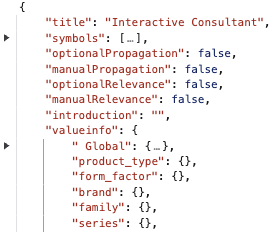
\includegraphics[width=\textwidth]{structuurJson.png}
        \caption[JSON-bericht]{\label{fig:structuurJson}Opbouw van meta en eval}
    \end{minipage}
    \hfill
    \begin{minipage}[b]{0.48\textwidth}
        \centering
        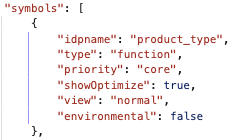
\includegraphics[width=\textwidth]{structuurSymbol.png}
        \caption[Symbool]{\label{fig:structuurSymbol}Structuur van symbool}
    \end{minipage}
\end{figure}

De JSON-berichten, meta en eval, hebben dezelfde structuur maar verschillen in inhoud. In deze studie wordt enkel gewerkt met de volgende twee elementen: \textit{symbols} en \textit{valueInfo}. De array \textit{symbols} bevat symbolen die elk een element \textit{idpname} bevatten. Deze woorden worden gebruikt om in de woordwolk weer te geven. In het eerste deel van deze fase krijgen de woorden een vaste, hardgecodeerde relevantie. Later worden de gewichten uit de databank opgehaald. Het element \textit{valueInfo} bevat informatie over de mogelijke en de actuele waarde van elk symbool.

\subsection{Integratie REST API en databank}
Om de gebruiker te helpen vinden wat hij zoekt, is het noodzakelijk om onderscheid te kunnen maken in de relevantie van woorden. Dit benadrukt de noodzaak van een REST API en een databank, aangezien dit met het huidige datamodel niet eenvoudig kan worden bijgehouden. Hiervoor worden twee tabellen aangemaakt: \textit{properties} en \textit{user\_interactions} (zie codefragment \ref{code:postgresql-tabellen}).
\begin{listing}
    \begin{minted}[
        frame=single,
        linenos,
        breaklines=true,
        fontsize=\small,
        baselinestretch=0.8
        ]{postgresql}
        CREATE TABLE properties ( 
        id INTEGER GENERATED ALWAYS AS IDENTITY PRIMARY KEY, 
        guinaam VARCHAR(100) NOT NULL, 
        relevantie INTEGER NOT NULL 
        );
        
        CREATE TABLE user_interactions (
        id INTEGER GENERATED ALWAYS AS IDENTITY PRIMARY KEY,
        propertyid INTEGER NOT NULL,
        timestamp TIMESTAMP NOT NULL DEFAULT CURRENT_TIMESTAMP,
        interaction_type INTEGER NOT NULL DEFAULT 0 
        CHECK (interaction_type IN (-2, 2)),
        FOREIGN KEY (propertyid) REFERENCES properties(id)
        );
    \end{minted}
    \caption{PostgreSQL-schema voor het creëren van de tabellen}
    \label{code:postgresql-tabellen}
\end{listing}
De REST API is een Node.js- en Express-server geschreven in TypeScript en draait op poort 3000. Er is bewust gekozen om de databank onafhankelijk op te zetten, zodat andere databankimplementaties eenvoudig kunnen worden toegevoegd zonder dat bestaande code aangepast hoeft te worden. In codefragment \ref{code:config/db} is te zien hoe de juiste databaseimplementatie wordt geselecteerd op basis van een omgevingsvariabele. De file \textit{postgres-db.ts} (zie codefragment \ref{code:config/postgres}) bevat de queries en databaselogica specifiek voor PostgreSQL. Deze implementeert de DatabaseInterface met concrete methoden voor het ophalen, aanmaken en bijwerken van gegevens in een PostgreSQL-database. Door deze implementatie te scheiden van de interface in \textit{database.ts} (zie codefragment \ref{code:types/database}), wordt het dus mogelijk om eenvoudig andere databasetypes toe te voegen zonder de rest van de applicatie aan te passen.
\begin{listing}
    \begin{minted}[
        frame=single,
        linenos,
        breaklines=true,
        fontsize=\small,
        baselinestretch=0.8
        ]{typescript}
        import { DatabaseInterface } from '../types/database';
        import postgresDb from './postgres-db';
        // Hier zou je andere database-implementaties kunnen importeren
        import dotenv from 'dotenv';
        
        dotenv.config();
        
        // Configureer welke database je wilt gebruiken op basis van omgevingsvariabele
        const dbType = process.env.DB_TYPE || 'postgres';
        
        let db: DatabaseInterface;
        
        switch (dbType) {
            case 'postgres':
            db = postgresDb;
            break;
            // Andere cases voor andere databases
            default:
            db = postgresDb; // Standaard als fallback
        }
        
        export default db;
    \end{minted}
    \caption{config/db.ts: bevat configuratie voor het type databank dat wordt gebruikt}
    \label{code:config/db}
\end{listing}

\begin{listing}
    \begin{minted}[
        frame=single,
        linenos,
        breaklines=true,
        fontsize=\small,
         baselinestretch=0.8
        ]{typescript}
        export interface DatabaseInterface {
            findByGuinaam(tableName: string, guinaam: string): Promise<any>;
            findByGuinaams(tableName: string, guinaams: string[]): Promise<any[]>;
            create(tableName: string, data: any): Promise<any>;
            findAll(tableName: string): Promise<any[]>;
            addUserInteractionSelectedPropertyToe(tableName: string, guinaam: string): Promise<any>;
            addUserInteractionUnselectedPropertyToe(tableName: string, guinaam: string): Promise<any>;
            increaseRelevanceProperty(tableName: string, guinaam: string): Promise<any>;
            decreaseRelevanceProperty(tableName: string, guinaam: string): Promise<any>;
        }
    \end{minted}
    \caption{types/database.ts: interface met de te implementeren methoden per type databank}
    \label{code:types/database}
\end{listing}

\begin{listing}
    \begin{minted}[
        frame=single,
        linenos,
        breaklines=true,
        fontsize=\small,
        baselinestretch=0.8
        ]{typescript}
        import { Pool, QueryResult } from 'pg';
        import { DatabaseInterface } from '../types/database';
        import dotenv from 'dotenv';
        import { PropertyModel } from '../types/property';
        
        dotenv.config();
        
        class PostgresDatabase implements DatabaseInterface {
            private pool: Pool;
            
            constructor() {
                this.pool = new Pool({
                    user: process.env.DB_USER,
                    host: process.env.DB_HOST,
                    database: process.env.DB_NAME,
                    port: parseInt(process.env.DB_PORT || '5432')
                });
            }
    \end{minted}
    \caption{config/postrgres-db.ts: een implementatie van de DatabaseInterface voor PostgreSQL. Het bevat de concrete logica voor het uitvoeren van database-operaties specifiek voor PostgreSQL. De concrete code is verschillend voor elk onderzoek.}
    \label{code:config/postgres}
\end{listing}

\paragraph{Synchroniseren woorden}
Wanneer de Interactive Consultant wordt ingeladen, wordt een HTTP-POST-request verstuurd naar http://localhost:3000/. In de frontend wordt de \textit{idpname} van de symbolen uit het meta-object gehaald, ontdaan van underscores en meegestuurd in het request naar de backend. Vervolgens worden de properties uit de databank opgehaald en vergeleken met de ontvangen symbolen. Symbolen die nog niet in de databank aanwezig zijn, maar wel in het request voorkomen, worden toegevoegd aan de tabel \textit{properties}. Het is belangrijk dat de symbolen uit het initiële meta JSON-bericht en die in de databank voortdurend gesynchroniseerd blijven

\paragraph{Ophalen gewichten van woorden}
Bij het toevoegen van een property aan de tabel \textit{properties} wordt de initiële relevantie van het bijbehorende woord op 15 gezet. Wanneer de renderfunctie van de woordwolk wordt aangeroepen, worden de properties met hun bijbehorende gewicht uit deze tabel opgehaald en toegewezen aan de array die wordt meegegeven aan de optie \textit{list} van de woordwolk.

\paragraph{Gebruikersinteractie registreren}
Om de voorkeuren van de gebruiker in kaart te brengen, moeten zijn of haar keuzes worden vastgelegd. Hiervoor wordt gekeken naar het element \textit{valueInfo} van de eval JSON-berichten. Zoals eerder vermeld, wordt het meta-object in de frontend telkens bijgewerkt wanneer er een nieuw JSON-bericht van de backend wordt ontvangen. Wanneer de gebruiker een waarde toekent aan een property, krijgt deze de status \textit{GIVEN}. Elke property start initieel met de status \textit{UNKNOWN}, en krijgt deze status ook terug wanneer de gebruiker de waarde reset. Om te achterhalen welke property werd gereset, wordt gekeken naar het element \textit{previousActive}, dat alle symbolen bevat met hun waarden en statussen. In de code worden zowel de \textit{GIVEN}-symbolen als de \textit{previousGIVEN}-symbolen bijgehouden in een array. Wanneer het meta-object verandert en het aantal \textit{GIVEN}-symbolen groter is dan dat van de \textit{previousGIVEN}-symbolen, kan worden geconcludeerd dat de gebruiker een waarde heeft toegekend aan een property. Vervolgens wordt gekeken welk symbool aanwezig is in de \textit{GIVEN}-array maar niet in de \textit{previousGIVEN}-array. Dit is de property waarvan de relevantie verhoogd moet worden. Hetzelfde principe geldt omgekeerd voor het verlagen van de relevantie wanneer een waarde wordt gereset. 

Om de gebruikersacties effectief te registreren wordt de tabel \textit{user\_interactions} gebruikt. Deze tabel registreert de volgende interacties:
\begin{itemize}
    \item \underline{Selecteren van een property}: het invullen van een waarde (relevantie +2)
    \item \underline{Deselecteren van een property}: het resetten van een waarde (relevantie -2)
\end{itemize}
Naast de \textit{propertyid} wordt ook het tijdstip van de interactie opgeslagen. Hierdoor kan de woordwolk periodiek worden bijgewerkt. Aan het einde van de dag worden alle interacties van die dag per property opgeteld en bij de bestaande relevantiewaarde in de tabel \textit{properties} gevoegd. Zo ontstaat er na verloop van tijd een beeld van welke properties het meest relevant zijn voor de gebruiker. Hoewel de periodieke updates niet volledig zijn uitgewerkt in deze studie, vormen ze een waardevolle uitbreiding van deze bachelorproef.

\paragraph{Relevantie rechtstreeks aanpassen}
De aanpak om de relevantie van properties te wijzigen, zoals hierboven beschreven, is niet geschikt voor een demo. Daarom wordt er best ook een demovriendelijke werkwijze uitgewerkt. In plaats van de gebruikersinteracties op te slaan in de tabel \textit{user\_interactions}, wordt de relevantie rechtstreeks aangepast in de tabel \textit{properties}. De logica om te bepalen welke property moet worden aangepast, blijft ongewijzigd. Het verschil zit in de uitvoering: er wordt eenvoudigweg een HTTP-POST-request verstuurd naar een ander endpoint.

\subsection{Styling van de woordwolk}
In dit onderzoek is de visuele uitstraling minstens even belangrijk als de implementatie van functionaliteit. Daarom wordt er gewerkt met kleuren en animaties. Volgende zaken worden verwerkt:
\begin{itemize}
    \item {Kleur van een property per categorie}
    \item {Uitleg over een property bij hoveren}
    \item {Kader rondom de property bij hoveren}
    \item {Achtergrondkleur van een \textit{consequency} property}
\end{itemize}
Om een overvloed aan kleuren te vermijden, krijgt elke property een kleur toegewezen op basis van de categorie. De unieke categorieën worden uit het meta-object gehaald en per sessie bijgehouden. Wanneer een gebruiker over een property hovert, verschijnt rechtsboven een tooltip met extra uitleg over de betreffende property (zie Figuur \ref{fig:tooltip}). Bij het hoveren wordt de property bovendien omkaderd in dezelfde kleur als die van de property zelf. Dit helpt de gebruiker om duidelijk te zien welke property hij mogelijk zal selecteren. \textit{CONSEQUENCE}-symbolen zijn properties waaraan de backend, het redeneersysteem, een waarde toekent als gevolg van een keuze van de gebruiker. Het invullen van een waarde bij een property kan dus gevolgen hebben voor de waarde van andere properties. Ook deze \textit{CONSEQUENCE}-symbolen worden uit het meta-object gehaald en bijgehouden in de webclient. Ze hebben de status \textit{CONSEQUENCE}. In de woordwolk worden deze symbolen weergegeven met een grijze achtergrondkleur (zie Figuur \ref{fig:consequence}).
\begin{figure}
    \centering
    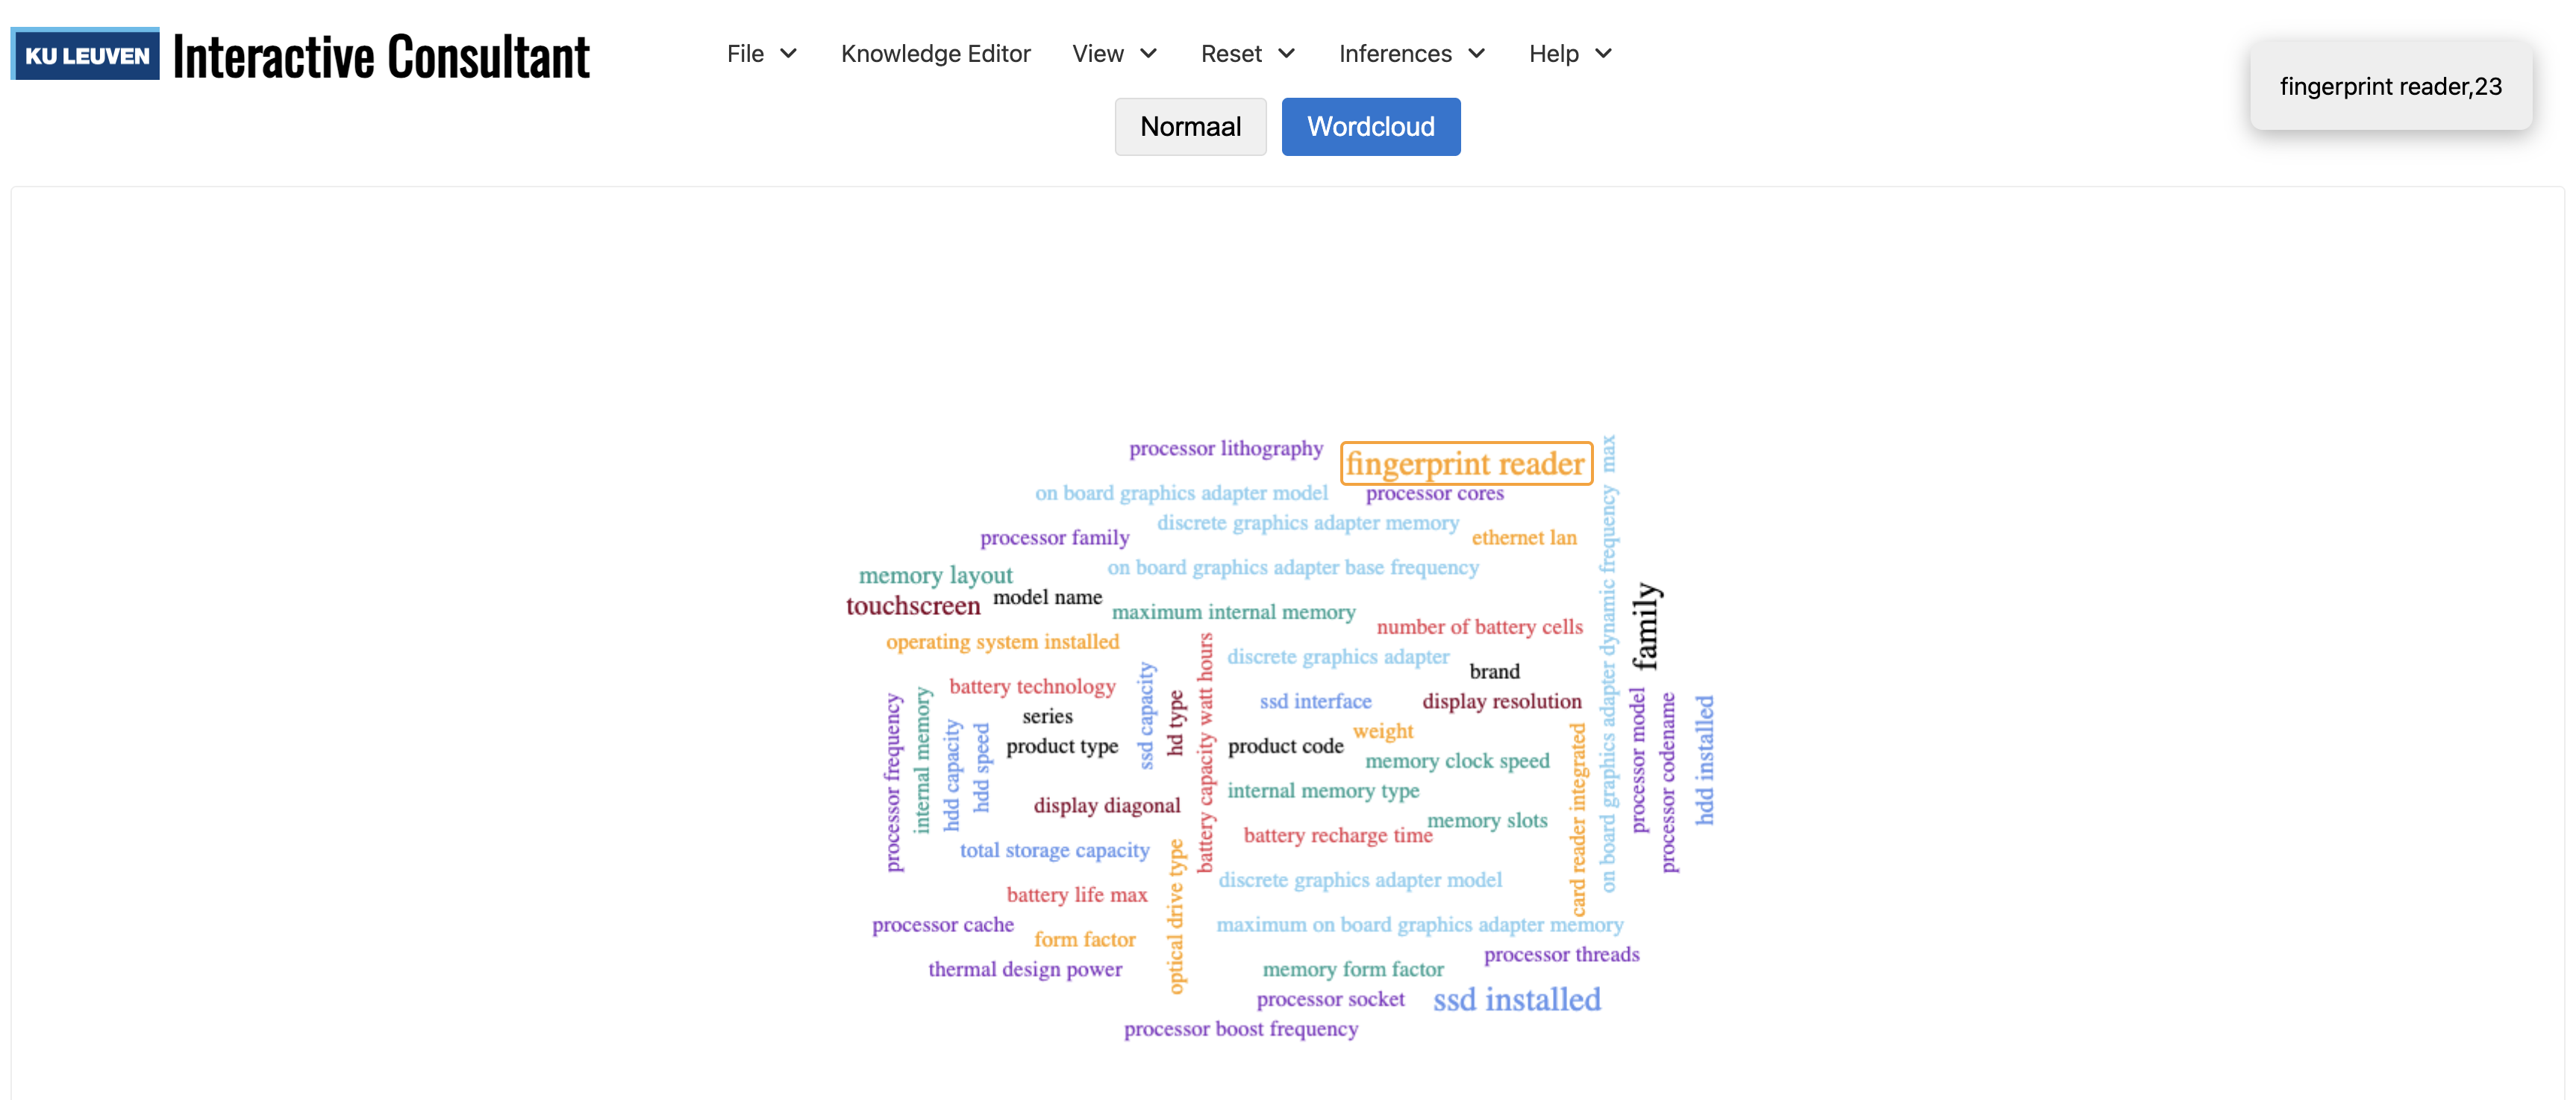
\includegraphics[width=1\textwidth]{tooltip.png}
    \caption[Styling bij het hoveren]{\label{fig:tooltip}De gehoverde property fingerprint reader wordt omrand in de bijbehorende kleur, en er verschijnt een tooltip met extra informatie over deze property.}
\end{figure}
\begin{figure}
    \centering
    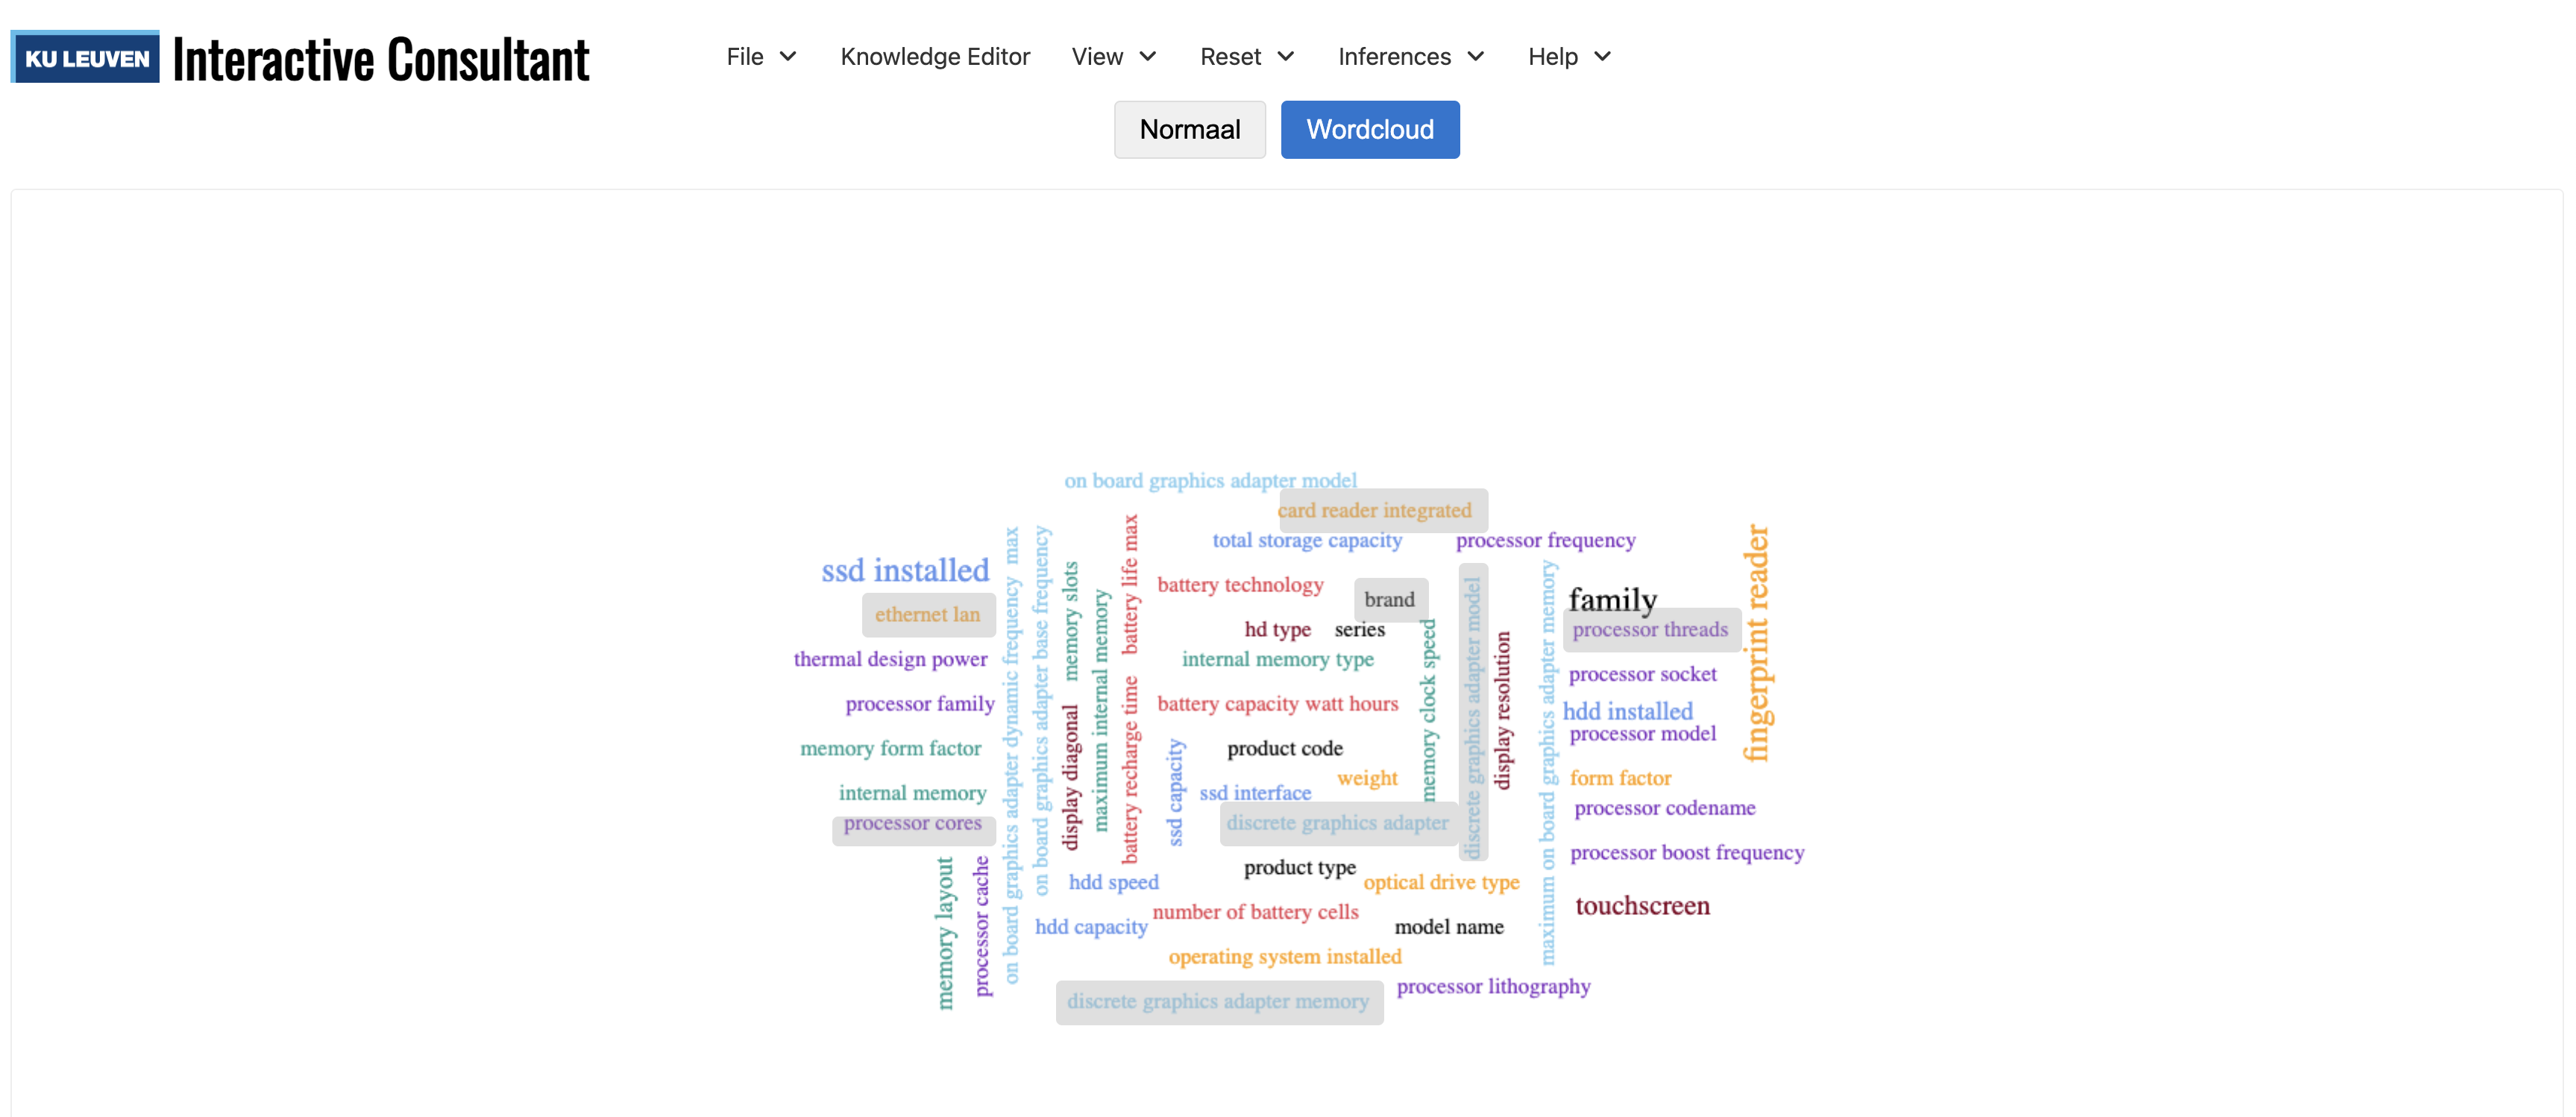
\includegraphics[width=1\textwidth]{consequence.png}
    \caption[Consequence-symbmolen]{\label{fig:consequence}De consequence-symbolen krijgen een grijze achtergrondkleur toegewezen.}
\end{figure}
\medskip\par Kaders en achtergrondkleuren zijn niet eenvoudig te implementeren, aangezien de posities van de woorden van de woordwolk niet standaard worden opgeslagen. Om dit probleem te omzeilen, worden muishover-events gesimuleerd waarbij de posities van de gehoverde properties worden opgeslagen.

\paragraph{Visuele resultaat proof-of-concept}
In dit onderdeel wordt het visuele resultaat van de proof-of-concept weergegeven. In Figuur \ref{fig:startscenario} is het startscenario van de webinterface te zien. Wanneer de applicatie voor de eerste keer wordt opgestart, krijgt elke property standaard dezelfde relevantiewaarde, namelijk 15.
\begin{figure}
    \centering
    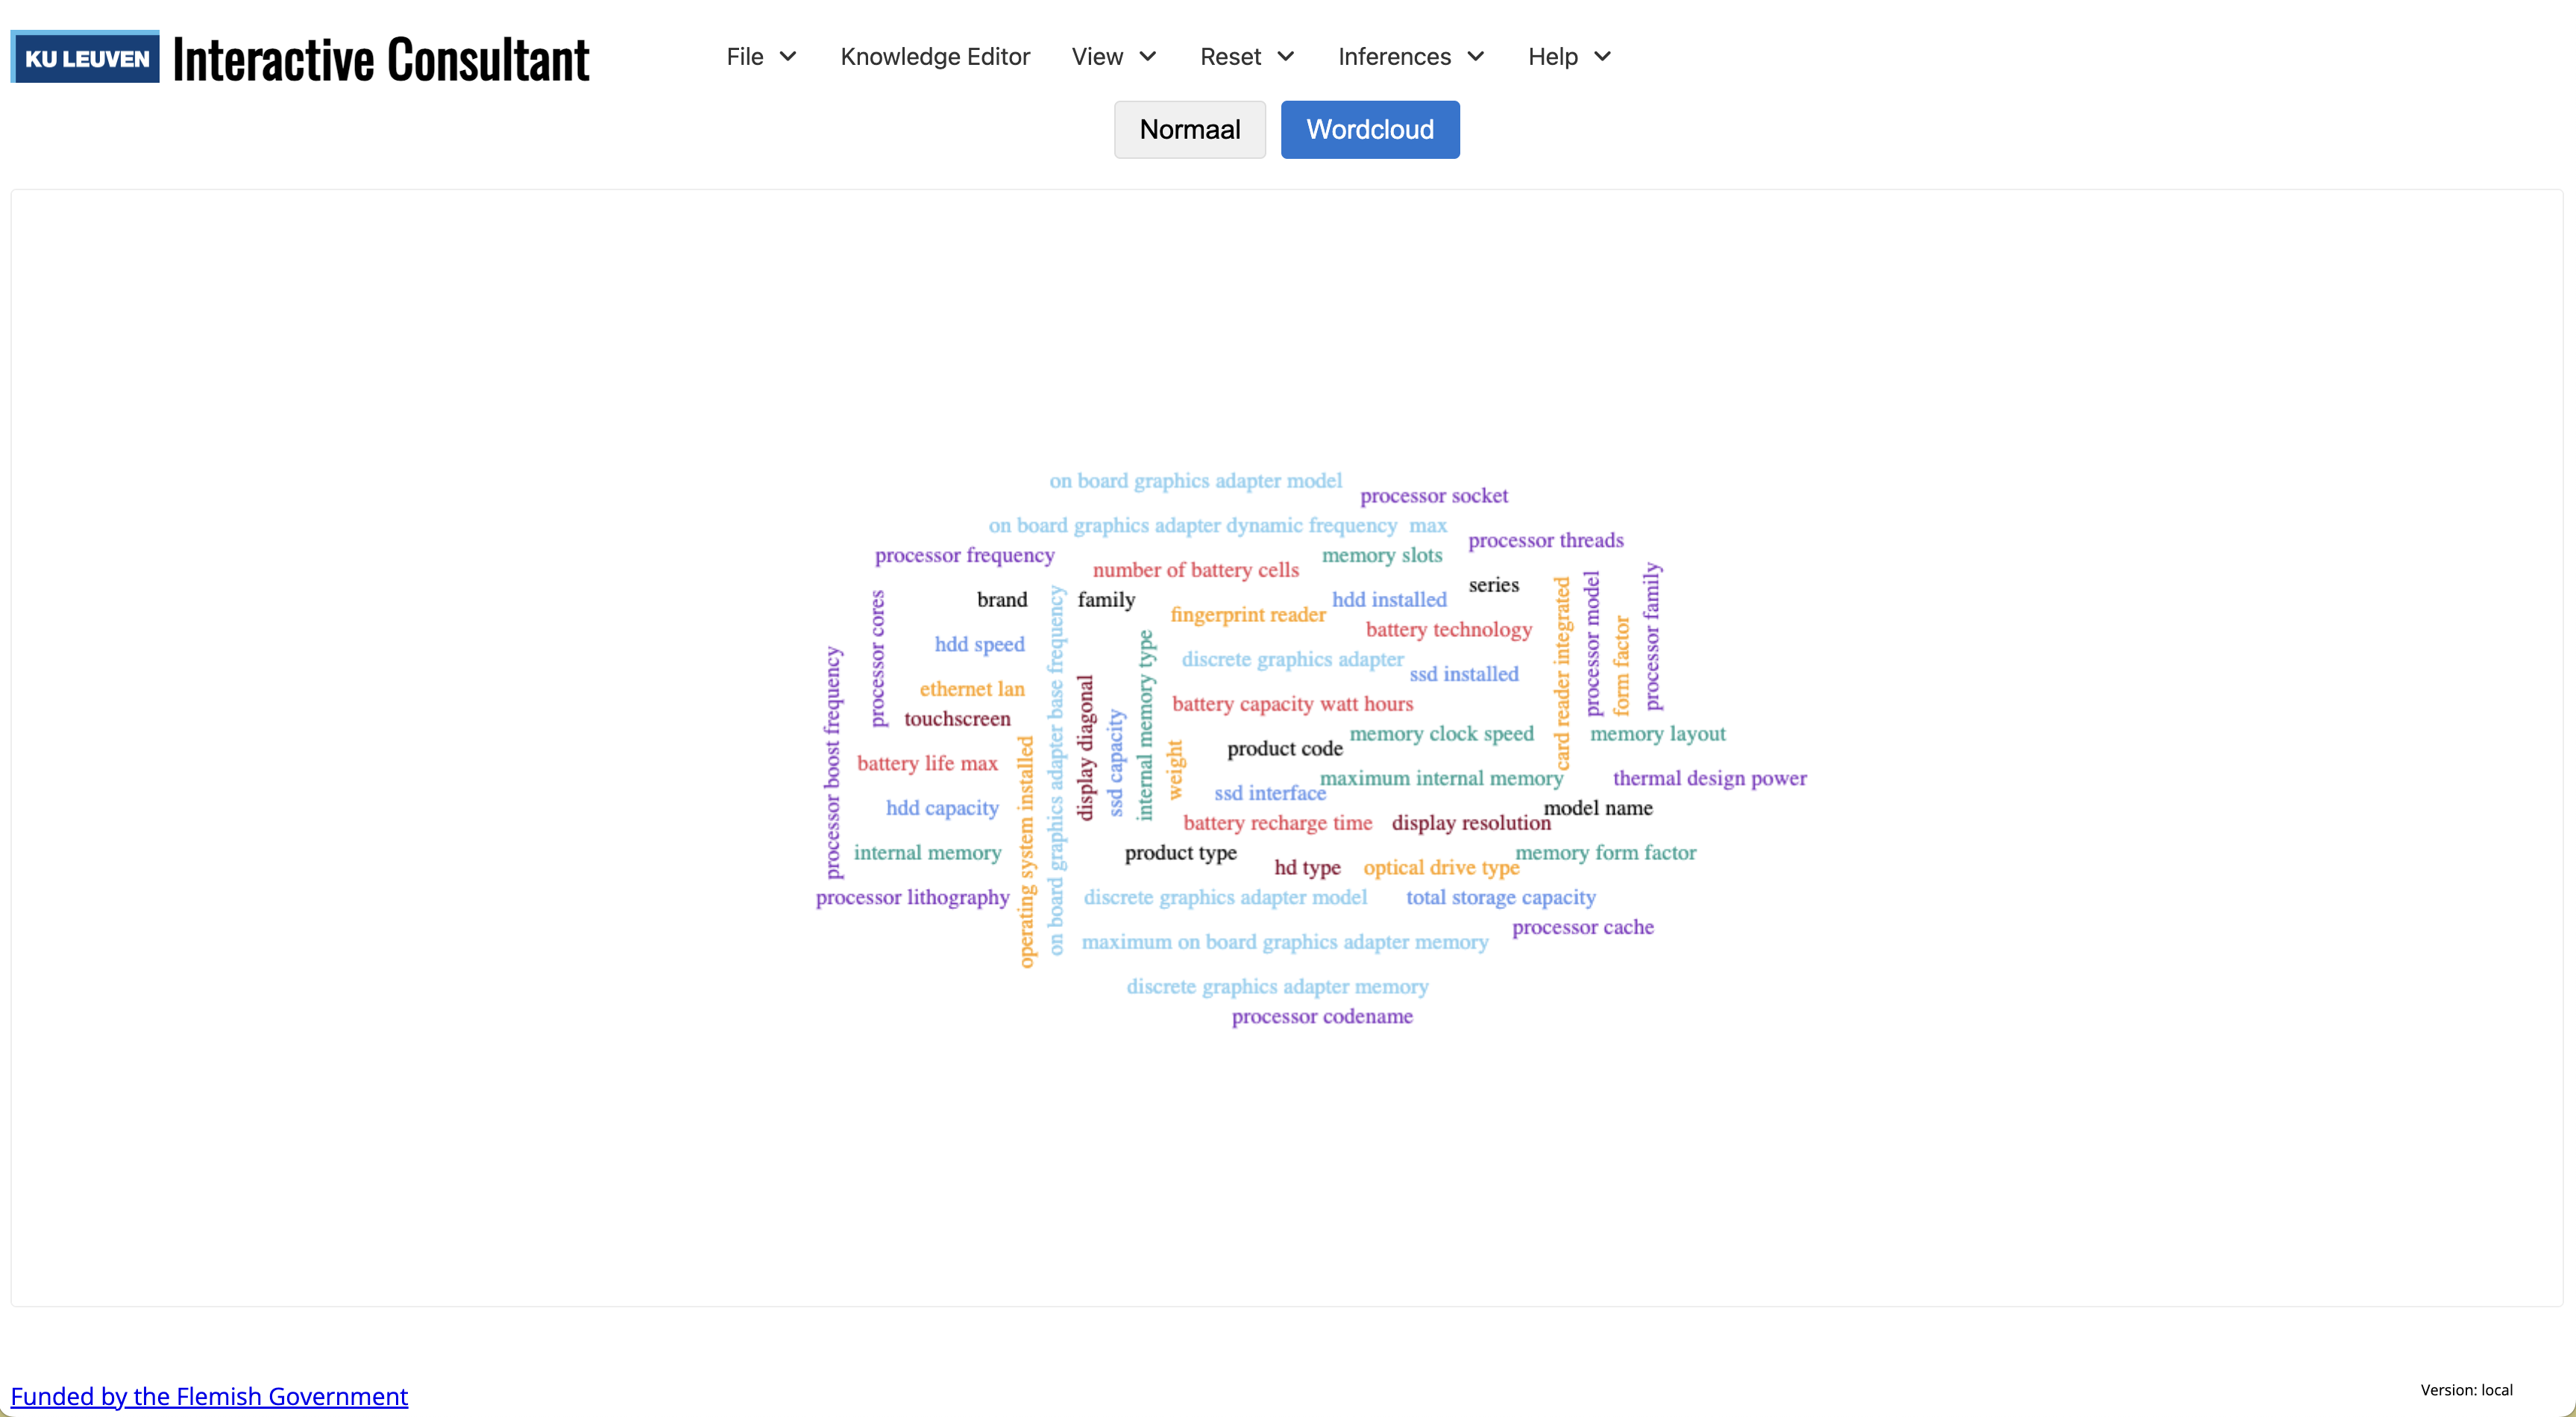
\includegraphics[width=1\textwidth]{startscenario.png}
    \caption[Startscenario webinterface]{\label{fig:startscenario}In het startscenario is de relevantie van elke property 15, wat resulteert in een woordwolk waarin alle woorden even groot worden weergegeven.}
\end{figure}
Figuur \ref{fig:doelscenario} is het beoogde scenario van deze bachelorproef. Het toont een mogelijke weergave van de woordwolk na langdurig gebruik. De belangrijkste properties voor de gebruikers zijn degene met de hoogste relevantiewaarde. Dit scenario wordt in de code gesimuleerd met de functie kenGewichtToe (zie codefragment \ref{code:kenGewichtToe}). Deze functie kent willekeurig een gewicht toe aan een woord, op basis van drie vooraf gedefinieerde gewichtscategorieën. De bijhorende code dient enkel ter illustratie en wordt verder niet gebruikt binnen de applicatie.
\begin{figure}
    \centering
    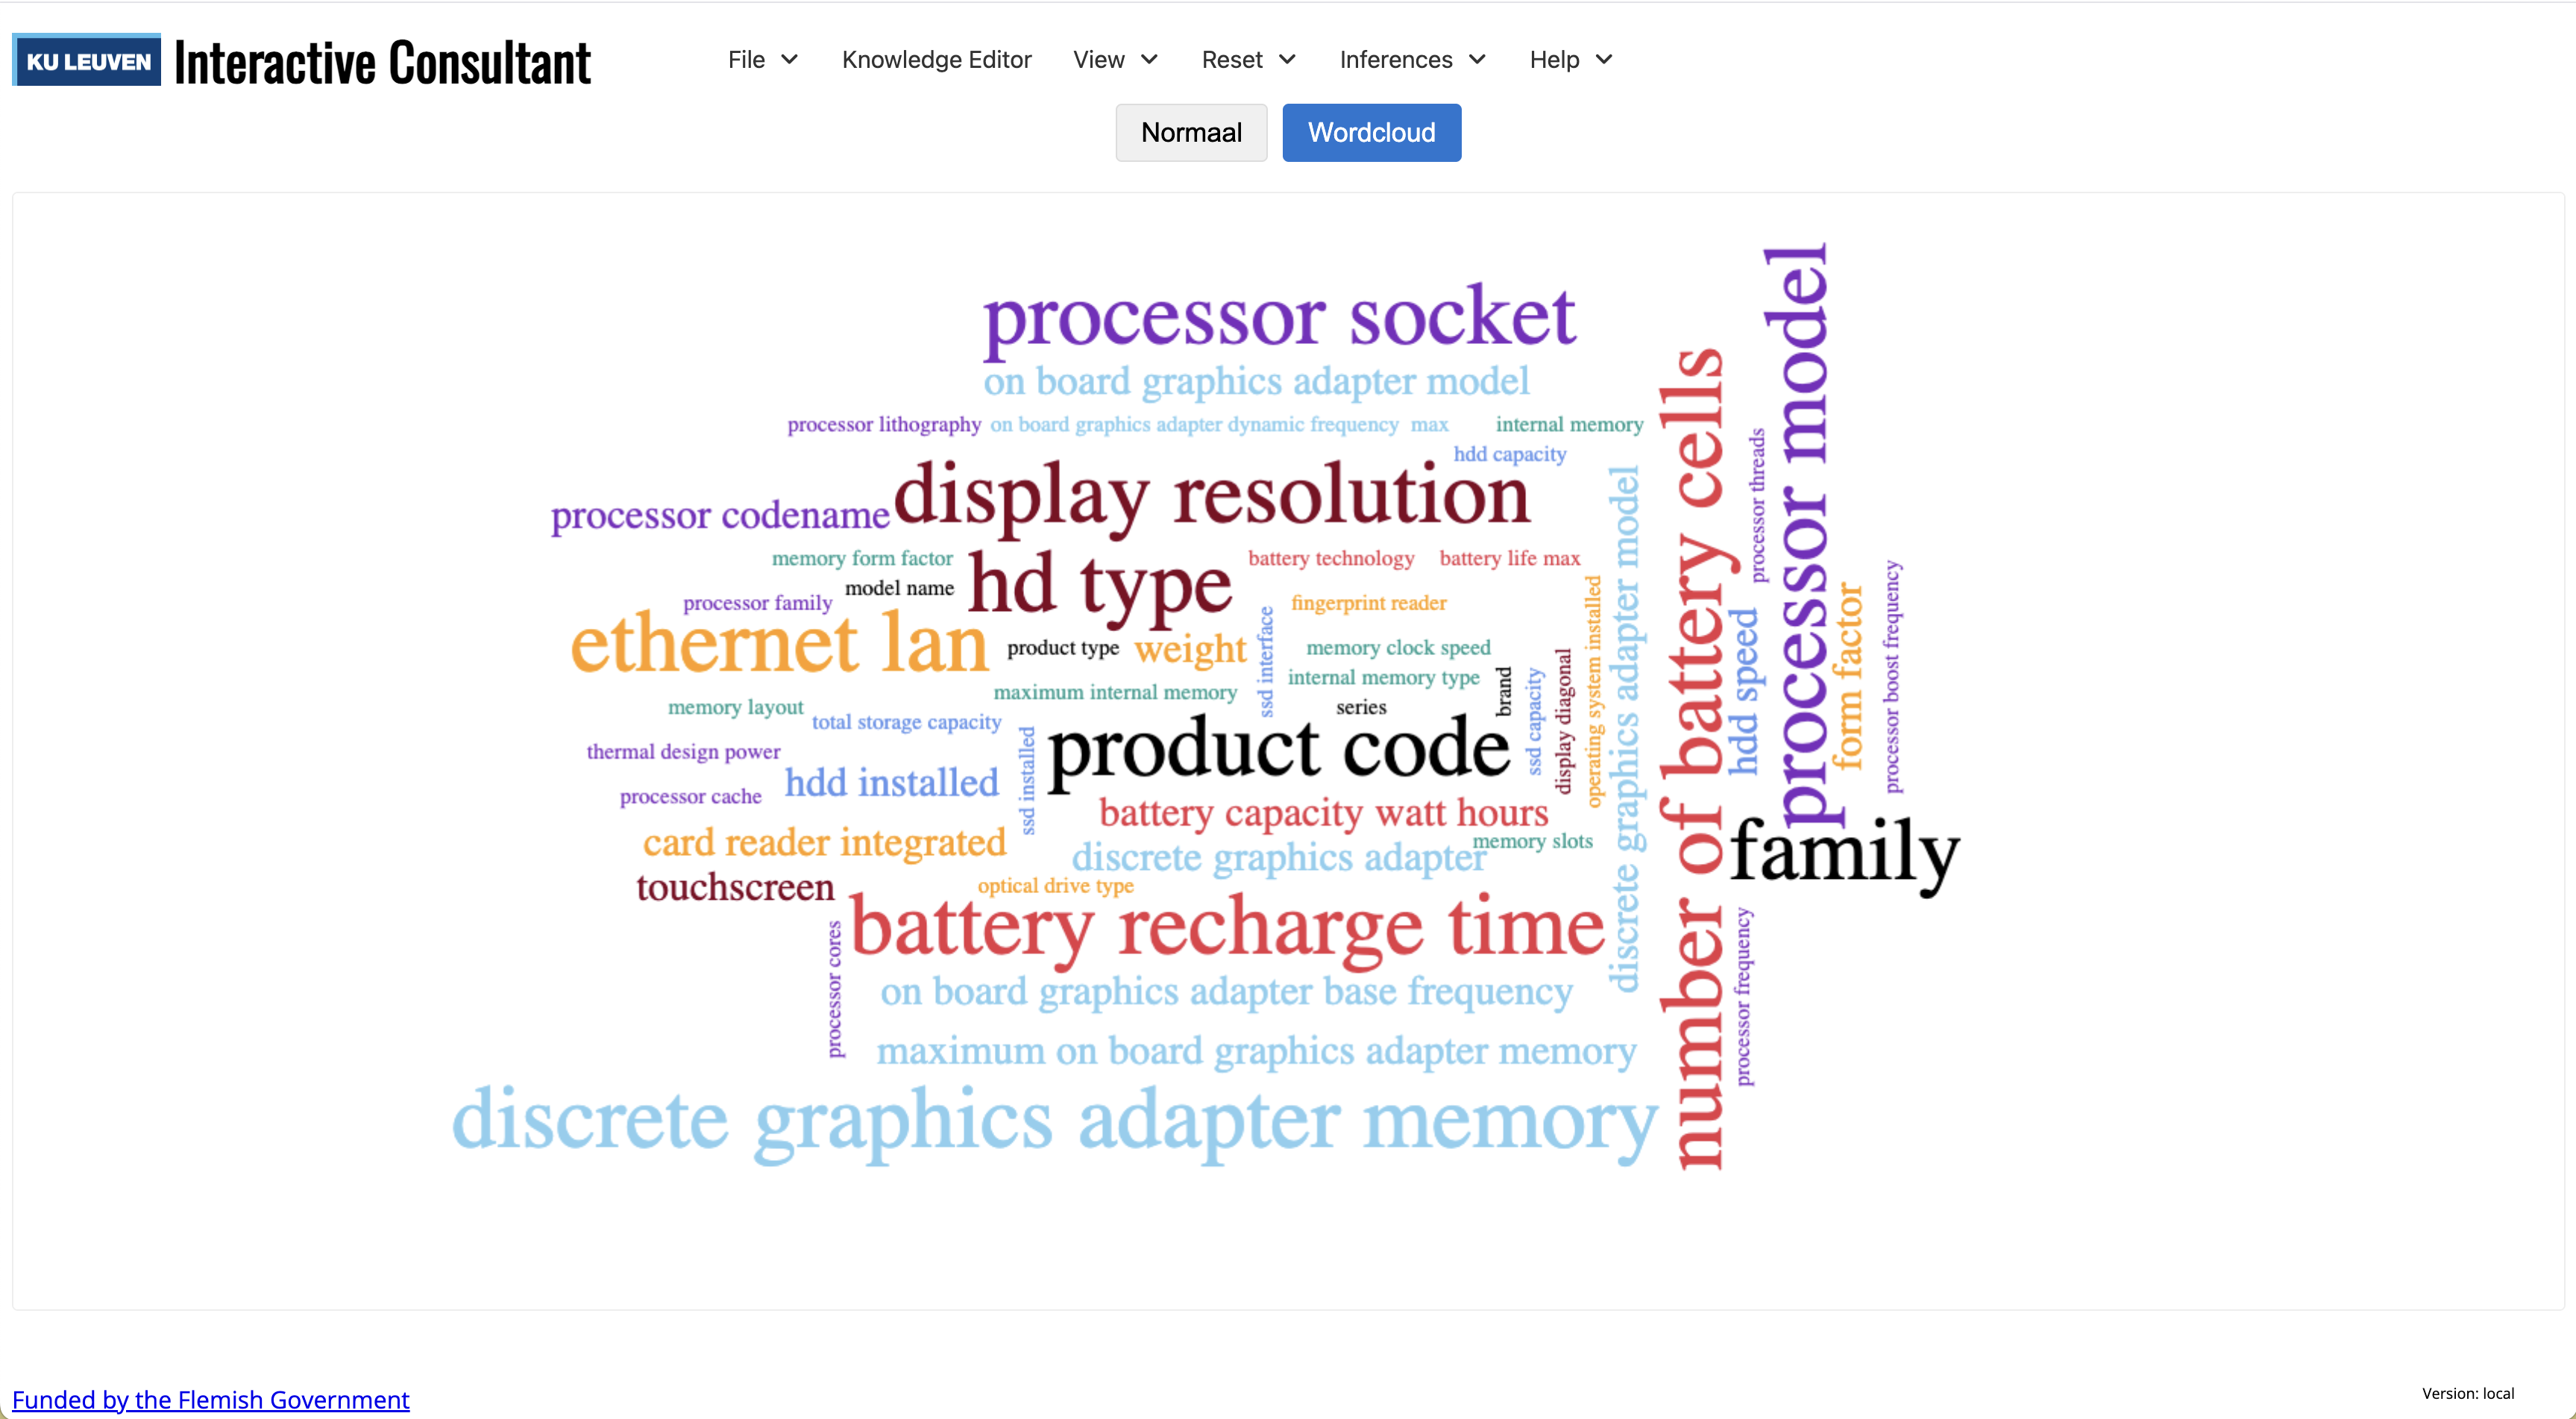
\includegraphics[width=1\textwidth]{doelscenario.png}
    \caption[Doelscenario webinterface]{\label{fig:doelscenario}In het doelscenario varieert de relevantie van de properties in functie van de interacties van de gebruiker.}
\end{figure}

\begin{listing}
    \begin{minted}[
        frame=single,
        linenos,
        breaklines=true,
        fontsize=\small,
        baselinestretch=0.8
        ]{typescript}
        kenGewichtToe(): number {
            const categorie1 = 15;
            const categorie2 = 28;
            const categorie3 = 60;
            
            const aantalWoorden = this.allSymbols.length;
            
            // Maximale aantallen per categorie
            const maxCategorie1 = Math.round(aantalWoorden * 0.50); // 50% van totaal
            const maxCategorie2 = Math.round(aantalWoorden * 0.35); // 35% van totaal
            const maxCategorie3 = Math.round(aantalWoorden * 0.15); // 15% van totaal
            
            // Bepaal welke categorie aan de beurt is
            if (this.categorie3Count < maxCategorie3 &&
            this.gewichtTeller % 5 === 0) {
                this.categorie3Count++;
                this.gewichtTeller++;
                return categorie3;
            } else if (this.categorie2Count < maxCategorie2 &&
            this.gewichtTeller % 3 === 1) {
                this.categorie2Count++;
                this.gewichtTeller++;
                return categorie2;
            } else if (this.categorie1Count < maxCategorie1) {
                this.categorie1Count++;
                this.gewichtTeller++;
                return categorie1;
            } else {
                // Als alle categorieën zijn opgebruikt, standaard naar categorie1
                return categorie1;
            }
        }
        \end{minted}
        \caption{De hulpmethode \textit{kenGewichtToe} verdeelt de woorden in drie categorieën met verschillende gewichten (15, 28 en 60) volgens een vastgelegde verhouding van 50\%, 35\% en 15\% van het totale aantal woorden. De toekenning gebeurt volgens een rotatiepatroon.}
        \label{code:kenGewichtToe}
    \end{listing}

\section{Conclusiefase}
De implementatie van de woordwolk-library WordCloud2.js voldoet aan alle requirements, op één na: het bijhouden en weergeven van de geselecteerde properties is nog niet uitgewerkt. Desondanks heeft deze technologie aangetoond een geschikte keuze te zijn voor het visualiseren van properties op een interactieve, dynamische en prioriteitsgestuurde manier. Ze vormt een significante verbetering ten opzichte van de huidige gebruikersinterface en biedt een verbeterde navigeerbaarheid en bruikbaarheid. Dit betekent echter niet dat dit de enige mogelijke optie is. Een nieuw prototype zou ontwikkeld kunnen worden met behulp van een andere eerder opgelijste library.

% Voeg hier je eigen hoofdstukken toe die de ``corpus'' van je bachelorproef
% vormen. De structuur en titels hangen af van je eigen onderzoek. Je kan bv.
% elke fase in je onderzoek in een apart hoofdstuk bespreken.

%\input{...}
%\input{...}
%...

%%=============================================================================
%% Conclusie
%%=============================================================================

\chapter{Conclusie}%
\label{ch:conclusie}

% TODO: Trek een duidelijke conclusie, in de vorm van een antwoord op de
% onderzoeksvra(a)g(en). Wat was jouw bijdrage aan het onderzoeksdomein en
% hoe biedt dit meerwaarde aan het vakgebied/doelgroep? 
% Reflecteer kritisch over het resultaat. In Engelse teksten wordt deze sectie
% ``Discussion'' genoemd. Had je deze uitkomst verwacht? Zijn er zaken die nog
% niet duidelijk zijn?
% Heeft het onderzoek geleid tot nieuwe vragen die uitnodigen tot verder 
%onderzoek?

Dit onderzoek toont aan dat het haalbaar is om informatie op een interactieve, dynamische en prioriteitsgestuurde manier te visualiseren met behulp van een front-end softwarebibliotheek. Een woordwolk biedt een efficiënte manier om een compacte en intuïtieve gebruikersinterface te ontwikkelen. De styling van deze visualisatie, zoals kleuren en tekstgroottes, verbeteren de navigeerbaarheid en bruikbaarheid van de interface.\medskip\par De vergelijkende studie geeft een duidelijk overzicht van de beschikbare visualisatietools. Aangezien elk alternatief voor- en nadelen heeft, is het moeilijk om slechts één ideale oplossing aan te wijzen. Het eindresultaat kan ook met andere alternatieven bereikt worden.
De huidige versie van het prototype vormt een sterke basis, maar biedt nog ruimte voor verbetering en uitbreiding. Om diepgaandere conclusies te kunnen trekken en om de relevante eigenschappen van de gebruikersinterface grondig te analyseren, moet het prototype van de laptop-demo gedurende een langere periode worden ingezet. Deze applicatie biedt een moderne, creatieve en intuïtieve weergave die interessant kan zijn voor bedrijven die op zoek zijn naar ondersteunende interfaces.

%---------- Bijlagen -----------------------------------------------------------

\appendix

\chapter{Onderzoeksvoorstel}

Het onderwerp van deze bachelorproef is gebaseerd op een onderzoeksvoorstel dat vooraf werd beoordeeld door de promotor. Dat voorstel is opgenomen in deze bijlage.

%% TODO: 
%\section*{Samenvatting}

% Kopieer en plak hier de samenvatting (abstract) van je onderzoeksvoorstel.

% Verwijzing naar het bestand met de inhoud van het onderzoeksvoorstel
%---------- Inleiding ---------------------------------------------------------
\section{Inleiding}%
\label{sec:inleiding}

Naast het creëren van een aangename gebruikerservaring spelen visuele effecten tijdens het navigeren op een website een significante rol in de communicatie van inhoud. Een woord dat getoond wordt, de kleur die daaraan wordt toegekend, de lettergrootte die wordt gekozen…~\autocite{Bordbar2016}. Al deze keuzes communiceren iets naar de bezoeker van de site. Volgens~\textcite{Lee2012} is de bruikbaarheid van een website een fundamenteel onderdeel van de gebruikerservaring. 

Deze studie richt zich op de online webIDE van het IDP-Z3 redeneersysteem van de KU Leuven. \textcolor{red}{De huidige gebruikersinterface van deze webIDE heeft overrompelt eindgebruikers met een ongestructureerde componenten en informatie. Het heeft een zwakke visuele uitstraling en kan een stuk verbeteren in bruikbaarheid en navigeerbaardheid.} De KU Leuven wil een nieuwe interface waarbij gebruikers snel en efficiënt kunnen navigeren naar wat ze nodig hebben. Het is de bedoeling dat de gebruikers geholpen worden in hun zoektocht naar de gewenste informatie.

%Hiervoor willen ze gebruik maken van een woordwolk. Volgens~\textcite{Atenstaedt2012} is een woordwolk een visuele weergave van woordfrequentie. Hoe vaker een term voorkomt in een dataset, hoe groter het woord verschijnt in de wolk.

Momenteel toont de huidige gebruikersinterface een opsomming van eigenschappen die gezien kunnen worden als filters. Elke filter heeft dezelfde opmaak en er wordt geen onderscheid gemaakt tussen relevante en minder relevante filters. Deze termen moeten op een andere manier gevisualiseerd worden en moeten kunnen reageren op realtime-interactie van de gebruiker. Via deze interactie kan er een prioriteit gekoppeld worden aan elke filter. De visualisatie van de dataset wordt vervolgens periodiek geüpdatet, zodat de filters die het meest aangeklikt worden, opvallender worden voor de eindgebruiker.

%Het probleem dat zich voordoet, is dat bestaande woordwolk-generatoren louter bedoeld\-zijn als ontwerptools. Ze kunnen niet omgaan met realtime veranderingen en bieden enkel opties aan voor het aanpassen van de typografie, kleur, woordoriëntatie en de vorm van de wolk \autocite{Heimerl2014}. De flexibiliteit en interactiviteit van deze derde-partijtoepassingen zijn te beperkt \autocite{Huang2019}. 

De centrale vraag van dit onderzoek is: \textcolor{blue}{Hoe kan een front-end softwarebibliotheek die informatie op een interactieve, dynamische en prioriteit gestuurde manier visualiseert, geïmplementeerd worden om structuur en duidelijkheid te creëren, zodat de navigeerbaarheid en bruikbaarheid van de IDP-Z3 webIDE van de KU Leuven verbeterd worden?} Verder worden er antwoorden gevonden op de volgende deelvragen:
\begin{itemize}
    \item \textcolor{green}{Op welke manier wordt de dataset in de huidige gebruikersinterface gevisualiseerd?}
    \item \textcolor{green}{Welke problemen heeft de huidige gebruikersinterface?}
    \item \textcolor{green}{Wat wordt bedoeld met bruikbaarheid en navigeerbaarheid van een website?}
    \item \textcolor{orange}{Welke visuele elementen spelen een rol in het verbeteren van de gebruikerservaring?}
    \item \textcolor{orange}{Wat zijn de belangrijkste vereisten voor de nieuwe gebruikersinterface?}
    \item \textcolor{orange}{Wat zijn de visualisatietools die kunnen gebruikt worden en welke is de meest toepasselijke?}
\end{itemize}

De methode die in deze studie gebruikt wordt, is het bouwen van een proof-of-concept voorafgegaan aan een vergelijkende studie. Er wordt een webapplicatie gebruikmakend van een softwarebibliotheek opgezet die communiceert met een REST API-server. Aan de hand van de require\-ments-analyse van de vergelijkende studie wordt er bepaald welke front-end softwarebibliotheek hiervoor het best past.

Het eerste deel van dit rapport omvat de bevindingen van de literatuurstudie, waar\-in een antwoord wordt geformuleerd op bepaalde deelvragen. Vervolgens wordt de methodologie beschreven en worden de verwachte resultaten gesch\-etst. Het laatste hoofdstuk behandelt de conclusie van dit onderzoek.

%---------- Stand van zaken ---------------------------------------------------

\section{Literatuurstudie}%
\label{sec:literatuurstudie}

\subsection [Esthetiek, hiërarchie en voorkeur]{Esthetiek, visuele hiërarchie en\\gebruikersvoorkeur}
Esthetiek is door de jaren heen op verschillende manieren gedefinieerd. Esthetiek kan worden omschreven als “de wetenschap van hoe dingen via de zintuigen worden herkend”~\autocite[p.~12]{Noponen2017}. Website-esthetiek speelt een cruciale rol bij het ondersteunen van de inhoud en functionaliteit van een website. Elk visueel element communiceert iets naar de gebruiker. Deze effecten mogen door webdesigners niet worden genegeerd; het is juist door inzicht te hebben in deze effecten dat communicatie kan worden beïnvloed. 
De functionaliteit van een website verwijst naar de gebruiksvriendelijke aspecten van de interface. Het belangrijkste doel van functionaliteit is het creëren van websites waar gebruikers snel en efficiënt de gewenste informatie kunnen terugvinden~\autocite{Thorlacius2007}. Het verkrijgen van de gewenste inhoud is op veel websites moeilijk. Dit probleem ontstaat wanneer een website niet aansluit bij de behoeften van de gebruikers, maar zich voornamelijk richt op de interne prioriteiten van de organisatie. Een andere oorzaak is dat de informatie op de website niet logisch gestructureerd is voor de gebruiker~\autocite{Bevan1997}.
De manier waarop een gebruiker met een webpagina interacteert, wordt beïnvloed door de visuele uitstraling van de pagina~\autocite{Michailidou2008}. Een aantrekkelijke compositie trekt de aandacht van de gebruiker en brengt de boodschap snel en duidelijk over. Een betekenisvol contrast tussen schermelementen, ruimtelijke groeperingen en het uitlijnen van de elementen draagt bij aan deze aantrekkingskracht en zijn aspecten van visuele hiërarchie\\ \autocite{Bhaskar2011}. 

Websitehiërarchie speelt een centrale rol in het structureren van informatie op websites en beïnvloedt hoe gebruikers zich op een website navigeren~\autocite{Djonov2007}. Uit het onderzoek van \textcite{Urano2021} blijkt dat hiërarchie in de grafische indeling gebruikers kan sturen in een voorgeschreven volgorde. Webdesigners gebruiken deze techniek om de gebruikerservaring te sturen. Dit principe wordt bijvoorbeeld gebruikt in kranten, waarbij een kop met groot, vetgedrukt lettertype de aandacht van de lezer trekt. In dergelijke gevallen bepaalt de redacteur welke informatie het belangrijkst is. Door het gebruik van grootte, kleur, contrast, positionering en typografie kunnen websites op een soortgelijke manier hun gebruikersinterface optimaliseren en de bruikbaarheid verbeteren\\\autocite{Raghavendra2024}.

Een cruciaal element van visuele hiërarchie is de juiste prioritering van informatie. Gebruikers kunnen op die manier snel de gewenste informatie terugvinden~\autocite{Raghavendra2024}. In dit onderzoek ligt de nadruk echter op het visualiseren en begrijpen van de prioriteiten van de gebruiker. Volgens~\textcite{Lee2010} is het essentieel om inzicht te verkrijgen in hoe gebruikers hun voorkeuren vormen. Gebruikersvoorkeur verwijst naar de keuze tussen alternatieven op basis van persoonlijke mening. Deze voorkeur is een weerspiegeling van de gevoelens en houding ten opzichte van de website en beïnvloedt ook het gedrag van de gebruiker op die website~\autocite{Lee2010}.

\subsection{Bruikbaarheid}
Bruikbaarheid, ook wel gebruiksvriendelijkhe\-id genoemd, kan omschreven worden als de mate waarin gebruikers een website als gemakkelijk ervaren om te gebruiken~\autocite{Dianat2019}. Volgens~\textcite{Dingli2014} kan bruikbaarheid beschouwd worden als een kwaliteitsattribuut.\\Het doel van bruikbaarheid is om gebruikers te helpen hun taken efficiënt uit te voeren. Voor gebruikers die weinig tijd hebben om een systeem te leren kennen en minder computerervaring hebben, is bruikbaarheid van groot belang~\autocite{Mazumder2014}. Een eenvoudig ontwerp dat voldoet aan de behoeften van de gebruiker zorgt ervoor een doelgerichte gebruiker hun taken snel en moeiteloos kunnen voltooien en draagt bij aan de gebruiksvriendelijkheid van de website~\autocite{Pearson2007}. Dit is exact waar de focus op ligt in dit onderzoek: het ontdekken van de noden van de gebruiker en de interface hierop afstemmen. Volgens~\textcite{Zachrison2022} wordt de eerste indruk van de bruikbaarheid vastgesteld door het kijken naar de grafische interface zonder er daadwerkelijk gebruik van te maken. Dit wordt de pre-use usability of de bruikbaarheid voor gebruik genoemd. In deze studie zal een nieuwe gebruikersinterface ontworpen worden met een positieve pre-use ability.

\subsection{Navigeerbaarheid}
Navigeerbaarheid, of navigatiegemak, verwijst naar de mate van moeite en tijd die een gebruiker nodig heeft om de gewenste informatie op een interface te vinden. Het is een cruciaal element voor de kwaliteit van een website en essentieel om ervoor te zorgen dat de gebruiker zich in controle voelt~\autocite{Zachrison2022}. Eenvoudige, efficiënte, gebruiksgerichte en flexibele navigatie helpt de gebruiker bij het bereiken van zijn doelen~\autocite{Pearson2007}. Door de filters in de nieuwe gebruikersinterface te prioriteren en visueel aan te passen, kan de gebruiker snel vinden wat hij nodig heeft.

%\subsection [Wat is een woordwolk?]{Wat is een woordwolk en waarom wordt deze gebruikt?}
%Zoals hierboven vermeld, is een woordwolk e\-en visuele weergave van woordfrequentie. Hoe vaker een term voorkomt in een dataset, hoe groter het woord verschijnt in de wolk. Het wordt vaak gebruikt als hulpmiddel om de focus van teksten te identificeren. Woordwolken worden gebruikt in het bedrijfsleven en de politiek om 
%bijvoorbeeld de inhoud van politieke toespraken te visualiseren~\autocite{Atenstaedt2012}. Volgens~\textcite{Filatova2016} zijn ze oorspronkelijk ontworpen om websites of posters aantrekkelijker te maken, maar ze kunnen ook in het onderwijs voorkomen. Een woordwolk kan studenten helpen hun leestijd te verkorten, hun schrijfvaardigheden te verbeteren en hun woordenschat uit te breiden. Daarnaast kunnen ze bijvoorbeeld ook gebruikt worden om nieuwe woordenschat te presenteren.
%
%Een woordwolk kan een duidelijk overzicht bi\-eden door de woorden die het vaakst voorkomen, zichtbaar te maken. Hiervoor wordt de lettergrootte van de woorden gekoppeld aan de wo\-ordfrequentie \autocite{Heimerl2014}. Meestal gebeurt dit op een statische manier, maar in deze studie wordt er voornamelijk gefocust om dit dynamisch te laten verlopen. \textcite{DePaolo2014} zegt dat een woordwolk nuttig kan zijn om grote hoeveelheden tekstgegevens te filteren zodat ze makkelijk te begrijpen zijn. Voor dit onderzoek is de hoeveelheid woorden constant en gaat het niet zozeer om de woorden. Volgens~\textcite{KABIR2020} helpt een woordwolk de gedachten van gebruikers te begrijpen. Naast het verbeteren van de klantervaring, worden gebruikers ondersteunt in het nemen van beslissingen op een klantgerichte manier.


% Voor literatuurverwijzingen zijn er twee belangrijke commando's:
% \autocite{KEY} => (Auteur, jaartal) Gebruik dit als de naam van de auteur
%   geen onderdeel is van de zin.
% \textcite{KEY} => Auteur (jaartal)  Gebruik dit als de auteursnaam wel een
%   functie heeft in de zin (bv. ``Uit onderzoek door Doll & Hill (1954) bleek
%   ...'')

% Je mag deze sectie nog verder onderverdelen in subsecties als dit de structuur van de tekst kan verduidelijken.

%---------- Methodologie ------------------------------------------------------
\section{Methodologie}%
\label{sec:methodologie}

\subsection [Verduidelijkingsfase huidige situatie]{Verduidelijkingsfase huidige geb\-ruikersinterface}
Vooraleer er een nieuwe gebruikersinterface kan ontwikkeld worden, moet de huidige situatie geanalyseerd worden. Dit omvat het in kaart brengen van de gebruikte frameworks, datamodel en de manier waarop data tussen de front-end en de back-end wordt verzonden.

\subsection{Requirements-analysefase}
Bij het ontwikkelen van een nieuwe gebruikersinterface is het belangrijk te weten waaraan deze moet voldoen. Hiervoor zullen stakeholders betrokken worden bij het formuleren van de vereisten. Vervolgens zullen deze geordend worden volgens prioriteit, gebruik makend van de MoSCoW-methode. Deze fase kan beschouwd worden als de start van de vergelijken\-de studie van beschikbare technologieën en bibliotheken.

\subsection {Long list fase}
Aan de hand van deze eisen en de informatie verzameld in de vorige fasen, zullen er potentiële front-end softwarebibliotheken worden gezocht en opgesomd. Hiervoor wordt de literatuur opnieuw geraadpleegd.

\subsection {Short list fase}
Vervolgens wordt de lijst met alle gevonden alternatieven uitgedund. Via een samenvattende tabel worden de meest geschikte front-end softwarebibliotheek geselecteerd.

\subsection{Architectuur van de applicatie}
Een softwarebibliotheek is niet voldoende om een webapplicatie te bouwen. De architectuur van de applicatie moet ook uitgetekend en besproken worden. Er zal bepaald worden welke technologieën de applicatie moet bevatten. Hieronder is een hypothetische opstelling omtrent de architectuur van de applicatie gegeven:

\begin{itemize} 
    \item \textbf{Frontend:} Dit framework zal afhangen van de gekozen front-end softwarebibliotheek. Deze moeten namelijk compatibel zijn.
    \item \textbf{Backend:} Dit framework zal afhangen van het gekozen front-end framework. Deze m\-oeten met elkaar kunnen communiceren. Er zal gebruik gemaakt worden van een REST API-server.
    \item \textbf{Database:} Voor het bepalen van et datamodel en de databank kan er gekeken worden naar de huidige technologieën, maar dit is niet noodzakelijk.
\end{itemize}

\subsection{Proof-of-concept bouwen}
Nadat alle technische keuzes gemaakt zijn, zu\-llen deze getest en uitgewerkt worden. Er zal een prototype gebouwd worden om te valideren dat de gekozen technologieën effectief werken en de problemen oplossen.

\subsection{Conclusiefase}
Na de proof-of-concept wordt er een aanbeveling gegeven over het beste mogelijke alternatief. Ook de overgebleven  aspecten die niet aanwezig zijn in een van de onderzochte opties worden geïdentificeerd.

%Hier beschrijf je hoe je van plan bent het onderzoek te voeren. Welke onderzoekstechniek ga je toepassen om elk van je onderzoeksvragen te beantwoorden? Gebruik je hiervoor literatuurstudie, interviews met belanghebbenden (bv.~voor requirements-analyse), experimenten, simulaties, vergelijkende studie, risico-analyse, PoC, \ldots?
%
%Valt je onderwerp onder één van de typische soorten bachelorproeven die besproken zijn in de lessen Research Methods (bv.\ vergelijkende studie of risico-analyse)? Zorg er dan ook voor dat we duidelijk de verschillende stappen terug vinden die we verwachten in dit soort onderzoek!
%
%Vermijd onderzoekstechnieken die geen objectieve, meetbare resultaten kunnen opleveren. Enquêtes, bijvoorbeeld, zijn voor een bachelorproef informatica meestal \textbf{niet geschikt}. De antwoorden zijn eerder meningen dan feiten en in de praktijk blijkt het ook bijzonder moeilijk om voldoende respondenten te vinden. Studenten die een enquête willen voeren, hebben meestal ook geen goede definitie van de populatie, waardoor ook niet kan aangetoond worden dat eventuele resultaten representatief zijn.
%
%Uit dit onderdeel moet duidelijk naar voor komen dat je bachelorproef ook technisch voldoen\-de diepgang zal bevatten. Het zou niet kloppen als een bachelorproef informatica ook door bv.\ een student marketing zou kunnen uitgevoerd worden.
%
%Je beschrijft ook al welke tools (hardware, software, diensten, \ldots) je denkt hiervoor te gebruiken of te ontwikkelen.
%
%Probeer ook een tijdschatting te maken. Hoe lang zal je met elke fase van je onderzoek bezig zijn en wat zijn de concrete \emph{deliverables} in elke fase?

%---------- Verwachte resultaten ----------------------------------------------
\section{Verwacht resultaat, conclusie}%
\label{sec:verwachte_resultaten}
Op basis van de literatuurstudie kan worden geconcludeerd dat de nieuwe gebruikersinterfa\-ce, met een positieve aangepaste visuele uitstraling en gestructureerde componenten, de bruikbaarheid en navigeerbaarheid kan verbeteren. \\Uit het onderzoek wordt verwacht dat een geschikte softwarebibliotheek wordt gevonden die in staat is de bevindingen uit de literatuur te bevestigen. Daarnaast wordt verwacht dat de factoren die de gebruikerservaring verbeteren, met succes kunnen worden toegepast op de interactieve, dynamische en prioriteit gestuurde visualisatie. Om tot een concrete conclusie te komen, is verder onderzoek noodzakelijk. De proof-of-concept moet verder worden ontwikkeld tot een volwaardige webapplicatie die over een langere periode kan worden ingezet binnen de KU Leu\-ven-omgeving.



%%---------- Andere bijlagen --------------------------------------------------
% TODO: Voeg hier eventuele andere bijlagen toe. Bv. als je deze BP voor de
% tweede keer indient, een overzicht van de verbeteringen t.o.v. het origineel.
%\input{...}

%%---------- Backmatter, referentielijst ---------------------------------------

\backmatter{}

\setlength\bibitemsep{2pt} %% Add Some space between the bibliograpy entries
\printbibliography[heading=bibintoc]

\end{document}
